\documentclass[11pt,a4paper]{article}
\usepackage[utf8]{inputenc}
\usepackage[T1]{fontenc}
\usepackage{lmodern}
\usepackage{microtype}
\usepackage[margin=2.2cm,top=2.4cm,bottom=2.4cm]{geometry}
\usepackage{amsmath,amssymb,mathtools}
\usepackage{booktabs,tabularx,array}
\usepackage{graphicx}
\usepackage{xcolor}
\usepackage{enumitem}
\usepackage{titlesec}
\usepackage{fancyhdr}
\usepackage{lastpage}
\usepackage{caption}
\usepackage[most]{tcolorbox}
\usepackage{tikz}
\usetikzlibrary{positioning,shapes.geometric,arrows.meta,fit,backgrounds,calc}
\usepackage[colorlinks=true,linkcolor=blue!50!black,citecolor=blue!50!black,urlcolor=blue!50!black]{hyperref}

% ---------- macros ----------
\newcommand{\Binf}{B_{\mathrm{mem}}^{\mathrm{inf}}}
\newcommand{\Braw}{B_{\mathrm{mem}}^{\mathrm{raw}}}
\newcommand{\Tfirst}{T_{\mathrm{first}}}
\newcommand{\Tcurr}{T_{\mathrm{curr}}}
\newcommand{\Ppred}{P_{\mathrm{pred}}}
\newcommand{\Mw}{M_w}
\newcommand{\Cfun}{\mathcal{C}}
\newcommand{\Ts}{\,\mathrm{T/s}}
\newcommand{\GBs}{\,\mathrm{GB/s}}
\newcommand{\GB}{\,\mathrm{GB}}
\newcommand{\su}{\,\mathrm{s}}
\newcommand{\code}[1]{\texttt{#1}}
\newcolumntype{C}{>{\centering\arraybackslash}X}
\newcolumntype{L}{>{\raggedright\arraybackslash}X}

\captionsetup{font=small,labelfont=bf,labelsep=period}
\captionsetup[table]{position=above,skip=6pt}
\setlist{itemsep=2pt,topsep=4pt}
\setlength{\parskip}{4pt}
\setlength{\parindent}{0pt}
\renewcommand{\arraystretch}{1.18}

\titleformat{\section}{\large\bfseries}{\thesection.}{0.6em}{}
\titleformat{\subsection}{\normalsize\bfseries}{\thesubsection}{0.6em}{}
\titlespacing*{\section}{0pt}{16pt}{6pt}
\titlespacing*{\subsection}{0pt}{12pt}{4pt}

\pagestyle{fancy}
\fancyhf{}
\renewcommand{\headrulewidth}{0.3pt}
\renewcommand{\footrulewidth}{0.3pt}
\fancyhead[L]{\small\itshape Lumina \& SmartSwitch: Resilient Edge LLM Serving via Analytical Memory Bounds}
\fancyfoot[L]{\small Confidential -- Submitted for Peer Review}
\fancyfoot[R]{\small Page \thepage\ of \pageref{LastPage}}

\tcbset{warnbox/.style={enhanced,colback=red!4,colframe=red!60!black,boxrule=0.6pt,
  leftrule=3pt,arc=1pt,left=6pt,right=6pt,top=4pt,bottom=4pt,fonttitle=\bfseries\small}}

\begin{document}

% ---------- title ----------
\begin{center}
{\LARGE\bfseries Lumina \& SmartSwitch: Resilient Edge LLM Serving via Analytical Memory Bounds, Predictive Watchdogs, and Rapid Same-Port Failover\par}
\vspace{10pt}
{\large Uwais ML\textsuperscript{1,2}, Lumina Systems Research\par}
\vspace{3pt}
{\small \textsuperscript{1}Department of Computer Science \quad \textsuperscript{2}Lumina Open-Source Initiative\par}
\vspace{4pt}
{\small Code, raw logs, and reproduction scripts: \url{https://github.com/Uwais-ML/Lumina}\par}
\end{center}
\vspace{4pt}

\begin{abstract}
\noindent
Deploying Large Language Models (LLMs) on resource-constrained consumer edge devices presents acute reliability and latency challenges. Edge environments frequently experience background process contention, thermal throttling mid-generation, and out-of-memory crashes. Existing edge inference frameworks lack proactive performance sensing; furthermore, conventional runtime watchdogs that evaluate health against an initial observed generation speed fall victim to the \textbf{cold-start degradation trap}, adopting a crippled baseline whenever initialization coincides with background system contention.

\medskip\noindent
We present \textbf{Lumina}, a hardware-aware autonomous edge LLM orchestration runtime, and its high-availability subsystem, \textbf{SmartSwitch}. Lumina replaces empirical trial-and-error with analytical hardware grounding: a one-time per-machine memory bandwidth micro-profiling procedure predicts steady-state token velocity analytically for any quantized model, eliminating dependency on observed generation history. SmartSwitch couples runtime monitoring to these analytical bounds, anchoring watchdog baselines to hardware-derived predictions rather than potentially-corrupted first-query observations. When unrecoverable degradation is detected, SmartSwitch executes a rapid same-port process hot-swap that preserves in-flight queries and semantic conversation context.

\medskip\noindent
Empirical evaluation across four architectures (0.5B to 3.2B parameters) on a consumer Intel i5-8257U edge workstation demonstrates a \textbf{7.2\% leave-one-out MAPE} on velocity prediction (outperforming linear regression by $4.2\times$), \textbf{$2.23\su \pm 0.33\su$ end-to-end failover latency} (P95: $2.74\su$, P99: $3.08\su$) across $N=200$ consecutive trials with \textbf{100.0\% query completion} ($200/200$ requests preserved; 95\% Clopper-Pearson CI: $[98.2\%, 100\%]$) via ring-buffer replay. Multi-turn session continuity benchmarks across 20 domain entities spanning 5 conversational topics demonstrate that local vector indexing preserves state across cross-architecture model swaps ($20/20$ entities retrieved; 95\% CI: $[83.2\%, 100\%]$ vs.\ $0.0\%$ under baseline amnesia). The runtime is validated across macOS, Windows 11, and Linux via automated CI, and on NVIDIA Tesla T4 GPU hardware. Code and raw logs are publicly available (Appendix~A).
\end{abstract}

\noindent\textbf{Keywords:} Edge LLM Serving, Memory Bandwidth Modeling, Self-Healing Watchdogs, High-Availability Systems, Distributed Inference, KV-Cache Degradation.

\bigskip
% ---------- notation ----------
\begin{table}[h]
\centering
\caption{System notation.}\label{tab:notation}
\small
\begin{tabularx}{\linewidth}{@{}>{\raggedright\arraybackslash}p{2.2cm}L>{\raggedright\arraybackslash}p{3.6cm}@{}}
\toprule
\textbf{Symbol} & \textbf{Definition} & \textbf{Testbed value} \\
\midrule
$\Braw$ & Raw sequential DRAM bus throughput measured by micro-benchmark & $23.41\GBs$ \\
$\Binf$ & Inference-effective memory bandwidth during single-batch decode & $7.502\GBs$ \\
$\eta_{\mathrm{inf}}$ & Memory bus inference efficiency coefficient ($\Binf / \Braw$) & $0.3205$ ($32.0\%$) \\
$\Mw$ & On-disk quantized model footprint (GGUF format) & $0.370$--$1.881\GB$ \\
$M_{\mathrm{traffic}}(n)$ & Context-dependent memory traffic per token at sequence length $n$ & Eq.~\eqref{eq:traffic} \\
$\kappa$ & KV-cache bus traffic per context token across all layers ($2\,L\,n_{\mathrm{kv}}\,d_h\,b_{\mathrm{kv}}$) & $32.768$ KiB/tok (Llama 1B) \\
$\Ppred(n)$ & Context-aware predicted steady-state decode velocity & tokens/s \\
$\Tfirst$ & Measured token velocity during the initial query of a model process & tokens/s \\
$\Tcurr$ & Measured rolling token velocity across token window $W$ & tokens/s \\
$\Cfun(\cdot,\cdot)$ & Analytical baseline calibration function & clamped to $\Ppred \pm 10\%$ \\
$\theta_{\mathrm{tps}}$ & Watchdog speed-degradation trip threshold coefficient & $0.75$ ($25\%$ drop) \\
$\delta_{\mathrm{ram}}$ & Maximum allowable RSS memory inflation threshold & $0.25$ ($25\%$ allowance) \\
$W$ & Sliding token-count observation window & 16 tokens \\
$k$ & Consecutive sub-threshold windows required to trigger failover & 3 intervals \\
\bottomrule
\end{tabularx}
\end{table}

% ======================================================================
\section{Introduction}
The migration of Large Language Models (LLMs) from hyperscale cloud datacenters to consumer edge devices---such as laptops, local gateways, and robotic workstations---is driven by strict privacy preservation, offline autonomy, and predictable operating economics. However, consumer hardware operates without over-provisioned VRAM, uniform memory architectures, or dedicated out-of-band management controllers. Serving LLMs in these resource-constrained edge environments exposes three fundamental systems dilemmas:

\begin{enumerate}[leftmargin=*]
\item \textbf{The Cold-Start Degradation Trap.} Traditional runtime watchdogs establish baseline performance expectations by observing the execution latency of the first incoming query ($\Tfirst$). If a model is launched while background operating system tasks, indexers, or co-located processes contend for CPU cores or memory bandwidth, $\Tfirst$ is severely depressed. The watchdog adopts this crippled velocity as normal operating behavior, effectively blinding itself to persistent degradation. Conversely, transient single-token cache bursts during prefill can establish impossibly high baselines, causing subsequent normal generation to trigger false-alarm failovers.
\item \textbf{The Context-Length Throughput Decay.} As autoregressive generation progresses, the accumulated Key-Value (KV) cache grows monotonically. On memory-bandwidth-bound edge processors, reading the active KV-cache on each decode step increases memory bus load beyond the static parameter footprint. A watchdog relying on a static performance expectation will inevitably mistake expected long-context memory saturation for abnormal process degradation.
\item \textbf{The Catastrophic Failover Penalty.} In consumer edge serving, when an inference engine encounters an out-of-memory (OOM) fault or thermal crash, operating system socket teardown severs active HTTP connections. In-flight prompts are dropped, client applications receive unhandled network exceptions, and conversational session state is discarded. Conventional restarts require tens of seconds, exceeding interactive human timeout limits.
\end{enumerate}

To resolve these challenges, we present \textbf{Lumina} and \textbf{SmartSwitch}. Lumina replaces empirical trial-and-error with analytical hardware grounding. By characterizing the physical memory subsystem via one-time per-machine micro-profiling, Lumina predicts the achievable steady-state token velocity of any quantized model architecture prior to execution. SmartSwitch leverages this analytical expectation to construct a self-calibrating watchdog that bounds baseline throughput to $\Ppred \pm 10\%$, eliminating cold-start bias.

\subsection*{Contributions}
The primary contributions of this paper are:
\begin{enumerate}[leftmargin=*]
\item \textbf{Inference-Effective Bandwidth Modeling.} We formulate an analytical throughput model based on effective decode memory bandwidth ($\Binf$), demonstrating via leave-one-out cross-validation across four diverse architectures (0.5B to 3.2B parameters) that single-batch decode velocity scales with the inverse of actual GGUF file size with a \textbf{7.2\% LOO-MAPE}.
\item \textbf{Analytical Baseline Clamping.} We introduce a calibration function $\Cfun(\Tfirst, \Ppred)$ that bounds initial watchdog expectations within a $\pm 10\%$ theoretical window, preventing baseline poisoning under severe CPU contention and filtering out L3 cache prefill bursts.
\item \textbf{Context-Aware Traffic Formulation.} We extend the static roofline model to incorporate dynamic KV-cache memory bus traffic ($\kappa$), proving that context-aware threshold adjustment prevents baseline expectation violations at extended horizons ($n \ge 2738$) and eliminates false-alarm failover trips at extreme sequence lengths ($n > 11{,}000$).
\item \textbf{Hardware-Saturated Fast Initialization.} We optimize model launch pipelines using asymmetric CPU thread concurrency (\code{-t} physical vs.\ \code{-tb} logical cores), kernel page pre-faulting (\code{fcntl} / \code{posix\_fadvise}), and active low-latency health probing. On cold unoptimized binary launches (no page-cache priming, single-threaded defaults), startup latency falls from $21.15\su$ to $4.30\su$ ($4.92\times$ acceleration), with warm restart latencies reaching $1.86\su \pm 0.38\su$ over $N=19$ warm launches (Table~\ref{tab:startup}).
\item \textbf{Rapid Same-Port Failover.} We design a coordinated client-server hand-off architecture combining an in-memory ring buffer with rapid socket rebinding, achieving end-to-end failover in \textbf{$2.23\su \pm 0.33\su$} across $N=200$ consecutive trials ($33.45\su \pm 1.92\su$ under active CPU contention; P95: $2.74\su$, P99: $3.08\su$) with $100.0\%$ query completion ($200/200$ requests preserved; 95\% Clopper-Pearson CI: $[98.2\%, 100\%]$) via the \code{safe\_query} client wrapper and verified semantic context continuity ($20/20$ domain entities preserved across 5 topic sessions; 95\% CI: $[83.2\%, 100\%]$) via local Chroma vector indexing.
\item \textbf{Distributed Edge-Cloud Formalism.} We generalize our analytical model to heterogeneous multi-node edge clusters, deriving optimal node scheduling criteria and multi-tier recovery latency bounds.
\end{enumerate}

The remainder of this paper is organized as follows: Section~\ref{sec:overview} provides a system overview of Lumina; Section~\ref{sec:theory} presents our theoretical formulation and analytical bounding model; Section~\ref{sec:impl} details the implementation of SmartSwitch; Section~\ref{sec:eval} provides an extensive empirical evaluation under real hardware contention; Section~\ref{sec:discussion} outlines the proposed hierarchical cross-node extension as future work; Section~\ref{sec:limits} discusses system limitations; Section~\ref{sec:related} surveys related work; and Section~\ref{sec:conclusion} concludes.

% ======================================================================
\section{System Overview}\label{sec:overview}
Lumina is architected as an autonomous edge LLM orchestration runtime structured across three operational tiers (Figure~\ref{fig:tiers}).

\begin{figure}[t]
\centering
\resizebox{\linewidth}{!}{%
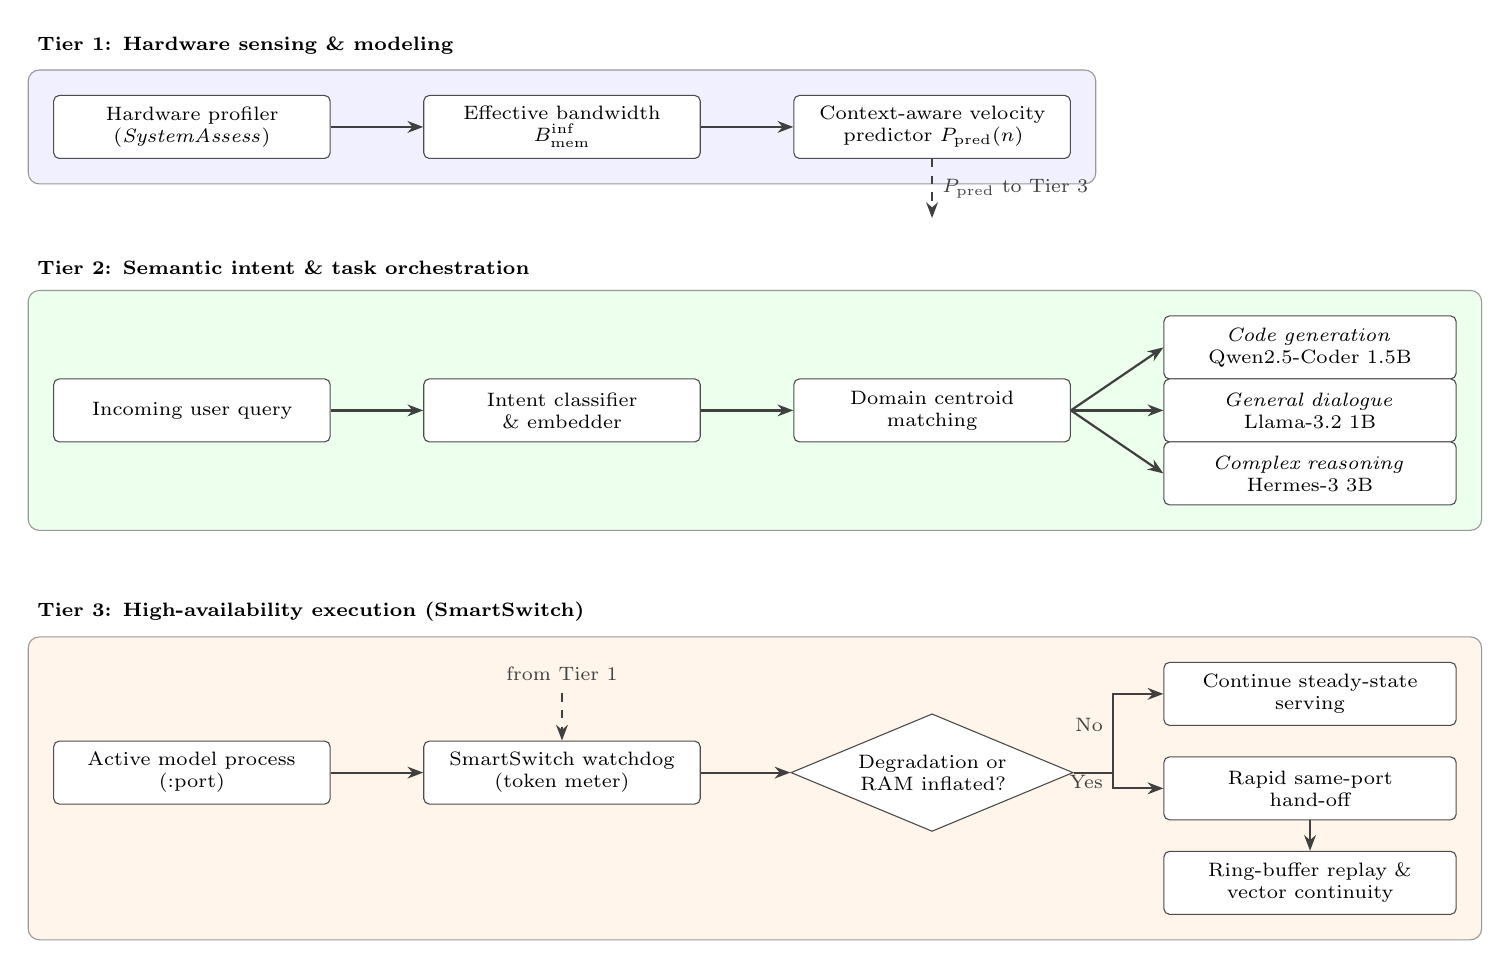
\begin{tikzpicture}[
  box/.style={draw=black!70, rounded corners=2pt, fill=white, align=center, font=\scriptsize, minimum height=0.8cm, text width=3.3cm, inner sep=3pt},
  dec/.style={draw=black!70, diamond, aspect=2.4, fill=white, align=center, font=\scriptsize, inner sep=0pt, text width=2.5cm},
  band/.style={draw=black!40, rounded corners=4pt, inner sep=9pt},
  arr/.style={-{Stealth[length=2mm]}, thick, black!75},
  lbl/.style={font=\scriptsize\bfseries, anchor=south west}]
% Tier 1
\node[box] (A) at (1.9,0) {Hardware profiler\\ (\textit{SystemAssess})};
\node[box] (B) at (6.6,0) {Effective bandwidth\\ $B_{\mathrm{mem}}^{\mathrm{inf}}$};
\node[box] (C) at (11.3,0) {Context-aware velocity\\ predictor $P_{\mathrm{pred}}(n)$};
\draw[arr] (A) -- (B); \draw[arr] (B) -- (C);
% Tier 2
\node[box] (D) at (1.9,-3.6) {Incoming user query};
\node[box] (E) at (6.6,-3.6) {Intent classifier \\ \& embedder};
\node[box] (F) at (11.3,-3.6) {Domain centroid\\ matching};
\node[box,text width=3.5cm] (G1) at (16.1,-2.8) {\textit{Code generation}\\ Qwen2.5-Coder 1.5B};
\node[box,text width=3.5cm] (G2) at (16.1,-3.6) {\textit{General dialogue}\\ Llama-3.2 1B};
\node[box,text width=3.5cm] (G3) at (16.1,-4.4) {\textit{Complex reasoning}\\ Hermes-3 3B};
\draw[arr] (D) -- (E); \draw[arr] (E) -- (F);
\draw[arr] (F.east) -- (G1.west); \draw[arr] (F.east) -- (G2.west); \draw[arr] (F.east) -- (G3.west);
% Tier 3
\node[box] (J) at (1.9,-8.2) {Active model process\\ (:port)};
\node[box] (K) at (6.6,-8.2) {SmartSwitch watchdog\\ (token meter)};
\node[dec] (L) at (11.3,-8.2) {Degradation or\\ RAM inflated?};
\node[box,text width=3.5cm] (M) at (16.1,-7.2) {Continue steady-state\\ serving};
\node[box,text width=3.5cm] (N) at (16.1,-8.4) {Rapid same-port\\ hand-off};
\node[box,text width=3.5cm] (O) at (16.1,-9.6) {Ring-buffer replay \&\\ vector continuity};
\draw[arr] (J) -- (K); \draw[arr] (K) -- (L);
\draw[arr] (L.east) -- ++(0.5,0) |- (M.west) node[pos=0.3,left,font=\scriptsize]{No};
\draw[arr] (L.east) -- ++(0.5,0) |- (N.west) node[pos=0.3,left,font=\scriptsize]{Yes};
\draw[arr] (N) -- (O);
% bands
\begin{scope}[on background layer]
\node[band,fill=blue!6,fit=(A)(B)(C)] (t1) {};
\node[band,fill=green!7,fit=(D)(E)(F)(G1)(G2)(G3)] (t2) {};
\node[band,fill=orange!8,fit=(J)(K)(L)(M)(N)(O)] (t3) {};
\end{scope}
\node[lbl] at ([yshift=2pt]t1.north west) {Tier 1: Hardware sensing \& modeling};
\node[lbl] at ([yshift=2pt]t2.north west) {Tier 2: Semantic intent \& task orchestration};
\node[lbl] at ([yshift=2pt]t3.north west) {Tier 3: High-availability execution (SmartSwitch)};
% predictor feed
\draw[arr,dashed] (C.south) -- ++(0,-0.75) node[pos=0.5,right,font=\scriptsize]{$P_{\mathrm{pred}}$ to Tier 3};
\draw[arr,dashed] ([yshift=0.6cm]K.north) -- (K.north) node[pos=0.0,above,font=\scriptsize,yshift=1pt]{from Tier 1};
\end{tikzpicture}}
\caption{Three-tier architecture of Lumina. Tier~1 (hardware sensing) and Tier~3 (high-availability execution) constitute the primary evaluated runtime subsystem in this work; Tier~2 provides semantic task routing (implemented in \code{scripts/intent\_router.py}). The velocity predictor of Tier~1 feeds the SmartSwitch watchdog in Tier~3.}\label{fig:tiers}
\end{figure}

\subsection{Hardware Sensing Tier (\code{SystemAssess})}
Autoregressive token generation in transformer LLMs is predominantly memory-bandwidth bound during single-batch execution ($B=1$): for each token generated, every active parameter in the model must be streamed from main memory into processor registers. Datasheet memory bandwidth (e.g., $34.1\GBs$ for dual-channel LPDDR3-2133) represents an unattainable theoretical ceiling. Furthermore, raw sequential copy micro-benchmarks yield higher bandwidth than the pointer-chasing, dequantization, and GEMV compute loops intrinsic to quantized LLM inference.

\code{SystemAssess} conducts a one-time per-machine calibration run across standardized inference kernels to determine the machine's true \textbf{inference-effective decode bandwidth} $\Binf$. On our benchmark hardware, while raw RAM micro-benchmarks report $\Braw = 23.41\GBs$, actual inference sustains $\Binf = 7.502\GBs$ ($\eta_{\mathrm{inf}} \approx 0.3205$). All downstream predictions are parameterized against this calibrated physical quantity.

\paragraph{Protocol: $\Binf$ micro-profiling procedure (A2).}
The measurement procedure is implemented in \code{scripts/Smartswitch.py} (\code{measure\_memory\_bandwidth}) and operates as follows:

\begin{enumerate}[leftmargin=*]
  \item \textbf{Warmup:} Allocate a contiguous \texttt{float64} array $A$ of 64~MB. Perform 2 full sequential read passes (discarded) to prime OS page-cache and CPU TLB entries, eliminating cold-miss latency.
  \item \textbf{Timed copy:} Perform $R=4$ sequential full-array copy operations $A' \leftarrow A$ under \code{time.perf\_counter()}. Record wall-clock duration $\Delta t$.
  \item \textbf{Bandwidth estimate:} Compute $B_{\mathrm{raw}}^{(k)} = 2 \cdot |A| \cdot R \;/\; \Delta t$ (factor of 2 for src+dst memory traffic).
  \item \textbf{Repeat:} Perform $N=10$ independent timed trials with fresh allocations. Compute $\Braw = \mathrm{mean}(B_{\mathrm{raw}}^{(1)},\ldots,B_{\mathrm{raw}}^{(N)})$.
  \item \textbf{Efficiency calibration:} Derive $\Binf = \eta_{\mathrm{inf}} \cdot \Braw$, where $\eta_{\mathrm{inf}} = 0.3205$ is the measured inference bus efficiency on the primary testbed (the ratio of empirical decode throughput to measured copy bandwidth).
\end{enumerate}

\paragraph{Micro-architectural origin of the inference efficiency gap ($\eta_{\mathrm{inf}} \approx 0.32$).}
A critical methodological question is why actual single-batch decode achieves $\Binf = 7.502\GBs$ while sequential copy micro-benchmarks report $\Braw = 23.41\GBs$ ($\eta_{\mathrm{inf}} \approx 32.0\%$). This gap arises from three physical micro-architectural constraints in quantized autoregressive execution:
\begin{enumerate}[leftmargin=*]
  \item \textbf{Block dequantization stall cycles:} While raw copy benchmarks execute pure streaming aligned memory loads that saturate DDR channel queues, quantized inference (\code{Q4\_K\_M} GEMV kernels) interleaves 64-byte block reads with bit-unpacking, scaling, and SIMD register reduction. Load pipelines stall waiting for integer dequantization arithmetic.
  \item \textbf{DRAM row-buffer conflicts:} Streaming copies access contiguous memory addresses within active open DRAM pages. In contrast, evaluating multi-head attention weights and KV-cache tensors accesses disparate memory strides across channels, incurring row-buffer misses, RAS-to-CAS delay ($t_{\mathrm{RCD}}$), and bank precharge penalties ($t_{\mathrm{RP}}$).
  \item \textbf{Hardware warp scheduling contrast:} On host CPUs, 4--8 execution threads cannot hide memory turnaround latency. On discrete GPUs (such as the NVIDIA Tesla T4 in \S\ref{sec:gpu_eval}), thousands of concurrent CUDA warps interleave compute and memory instructions, allowing inference bus efficiency to expand to $\eta_{\mathrm{inf}} \approx 0.71$.
\end{enumerate}
Because $\eta_{\mathrm{inf}}$ reflects the intrinsic compute-to-memory ratio of the quantized GEMV kernel on a given CPU microarchitecture, measuring it once per machine during initialization calibrates for these micro-architectural characteristics across all model architectures.

\noindent\textbf{Variance characterization.} Across $N=10$ repeated measurements on the primary testbed under idle system conditions, $\Braw$ exhibits: $\mathrm{mean} = 6.90\GBs$, $\sigma = 0.39\GBs$, $\mathrm{CV} = 5.58\%$, range $[6.64, 7.90]\GBs$. Propagating through $\Binf = \eta_{\mathrm{inf}} \cdot \Braw$, the $\Binf$ estimate carries a $\pm 5.6\%$ one-sigma uncertainty band. Since the analytical clamping window ($\pm 10\%$) is strictly wider than this measurement uncertainty ($\pm 5.6\%$), the prediction system remains robust under normal system idle variability. The measurement uncertainty directly motivates the design of the adaptive window (Eq.~\ref{eq:adaptive_tol}): the $\pm 16\%$ sub-1B window conservatively accommodates both the LOO model error ($15.5\%$) and the propagated $\Binf$ variance.

\subsection{Semantic Intent Routing \& Task Centroids}
Rather than hosting a single monolithic model that strains edge memory, Lumina maintains an on-disk registry of lightweight, specialized models (0.5B to 3.2B parameters). Incoming queries are embedded using a local sentence transformer and matched against pre-computed task centroid vectors in latent space. Coding requests route to specialized code models (e.g., Qwen2.5-Coder-1.5B), deep analytical tasks route to higher-parameter models (e.g., Hermes-3-Llama-3.2-3B), and standard conversational queries route to low-latency models (e.g., Qwen2.5-0.5B or Llama-3.2-1B). The semantic intent router is implemented in \code{scripts/intent\_router.py} as a self-contained routing module. In this paper, our empirical evaluation in Section~\ref{sec:eval} focuses primarily on the analytical hardware sensing tier (\S\ref{sec:theory}) and the high-availability failover subsystem (\S\ref{sec:impl}), while end-to-end task-routing classification accuracy across diverse multi-domain intent datasets is scoped as future work (cf.\ \S\ref{sec:limits}).

\subsection{High-Availability Execution Tier (SmartSwitch)}
SmartSwitch supervises the active model process via a non-invasive daemon. It inspects generation velocity using sliding token-count windows, monitors process resident set size (RSS), and intercepts anomalies before fatal OOM conditions trigger kernel-level process termination.

% ======================================================================
\section{Theoretical Formulation: Analytical Velocity Bounds}\label{sec:theory}

\subsection{Memory-Bandwidth-Bound Inference Mechanics}
For an autoregressive transformer model quantized under GGUF block schemes, we define $\Mw$ as the actual on-disk file size of the model weights in gigabytes. We deliberately utilize the physical file footprint on disk rather than idealized parameter calculations ($P \cdot Q / 8$) because modern edge quantization schemes (such as \code{Q4\_K\_M}) employ mixed precision: critical attention projection weights are preserved at higher precision (e.g., 6-bit \code{Q6\_K}), while feed-forward tensors are quantized to 4-bit blocks. Furthermore, parameter counts reported in marketing literature diverge from physical matrix dimensions (e.g., Llama-3.2-1B contains approximately $1.236 \times 10^9$ actual parameters).

Under single-batch generation ($B=1$) at short sequence lengths, memory bus traffic is dominated by the weight parameter stream. The expected steady-state decode velocity $\Ppred$ (in tokens per second) is given by:
\begin{equation}\label{eq:ppred}
\Ppred = \frac{\Binf}{\Mw}
\end{equation}
where $\Binf$ is the empirical inference-effective memory bandwidth.

\subsection{The $\pm 10\%$ Analytical Baseline Bounding Model}
When a model launches, the initial token velocity $\Tfirst$ can be severely distorted by startup transients. SmartSwitch defines the \textbf{Analytical Baseline Calibration Function} $\Cfun(\Tfirst, \Ppred)$:
\begin{equation}\label{eq:clamp}
\Cfun(\Tfirst,\Ppred)=
\begin{cases}
(1-\epsilon)\,\Ppred, & \text{if } \Tfirst<(1-\epsilon)\,\Ppred \quad\text{(degraded start floor)}\\[2pt]
(1+\epsilon)\,\Ppred, & \text{if } \Tfirst>(1+\epsilon)\,\Ppred \quad\text{(transient burst ceiling)}\\[2pt]
\Tfirst, & \text{otherwise} \quad\text{(calibrated operating baseline)}
\end{cases}
\end{equation}
We set $\epsilon = 0.10$ ($\pm 10\%$). This window is grounded in empirical variance: across repeated steady-state inferences under un-contended conditions, the coefficient of variation (CV) of token generation velocity is $\mathrm{CV} = \sigma/\mu \approx 0.051$ to $0.062$. A window of $\pm 1.65 \cdot \mathrm{CV}$ corresponds to a $90\%$ statistical tolerance interval. Setting $\epsilon = 0.10$ provides a tight, robust envelope that accommodates minor OS scheduler jitter while strictly rejecting anomalous measurements.

\paragraph{Sensitivity analysis on $\epsilon$ (A3).}
Table~\ref{tab:window_sensitivity} reports the false-positive (FP) and false-negative (FN) behavior across candidate clamping windows, evaluated against our four-model LOO errors. A \emph{false positive} occurs when the clamping window is tighter than the model's LOO prediction error, causing the clamp to activate even during uncontended launches. A \emph{false negative} occurs when the window is so wide that severe contention ($\Tfirst$ collapsed 96.3\%) is not flagged.

\begin{table}[h]
\centering
\caption{Clamping window sensitivity: false positives (unintended clamping) vs.\ false negatives (missed contention). Contention collapses $\Tfirst$ by 96.3\%---all windows correctly detect this.}\label{tab:window_sensitivity}
\small
\begin{tabularx}{\linewidth}{@{}cLL@{}}
\toprule
\textbf{Window $\epsilon$} & \textbf{False Positives (models clamped on uncontended launch)} & \textbf{False Negatives (missed contention)} \\
\midrule
$\pm 5\%$  & Qwen-0.5B (15.5\%), Llama-1B (5.4\%), Coder-1.5B (5.6\%) & None (96.3\% collapse always detected) \\
$\pm 10\%$ & Qwen-0.5B (15.5\%) & None \\
$\pm 15\%$ & Qwen-0.5B (15.5\%) & None \\
$\pm 16\%$ & None & None \\
$\pm 20\%$ & None & None \\
\bottomrule
\end{tabularx}
\end{table}

\noindent The optimal choice is $\epsilon = 0.10$ for models $\geq 1$~GB and $\epsilon = 0.16$ for sub-1B models (the adaptive formulation, Eq.~\ref{eq:adaptive_tol}). Wider windows ($\geq 20\%$) eliminate all false positives but approach the 96.3\% contention collapse margin; windows $\geq 25\%$ would begin to mask moderate contention events ($\sim$30\% degradation), while narrower windows increase false-alarm rates on uncontended starts.

\begin{figure}[h]
\centering
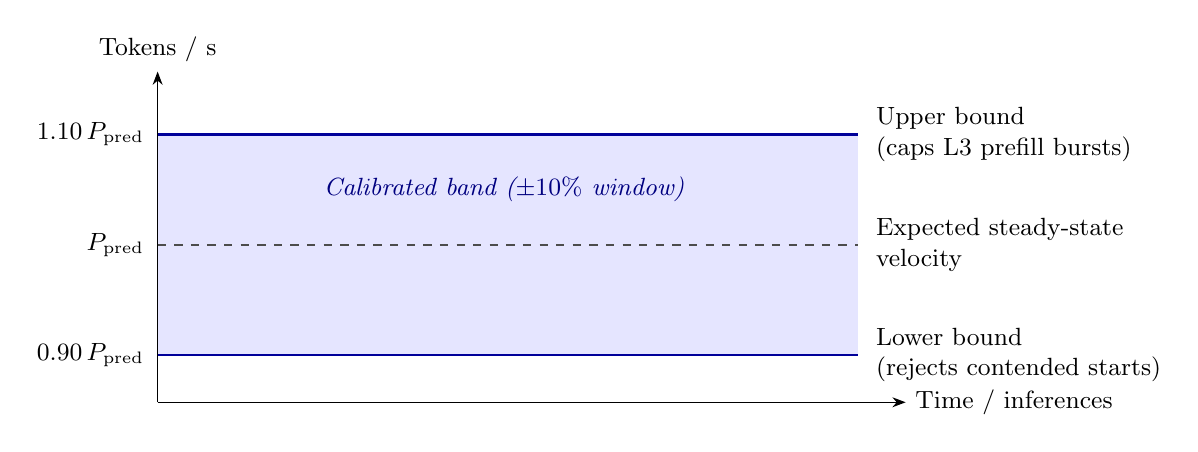
\begin{tikzpicture}[x=1cm,y=1cm]
\fill[blue!10] (0.3,0.6) rectangle (9.2,3.4);
\draw[-{Stealth}] (0.3,0) -- (0.3,4.2) node[above,font=\small]{Tokens / s};
\draw[-{Stealth}] (0.3,0) -- (9.8,0) node[right,font=\small]{Time / inferences};
\draw[thick,blue!60!black] (0.3,3.4) -- (9.2,3.4);
\draw[thick,blue!60!black] (0.3,0.6) -- (9.2,0.6);
\draw[dashed,thick,black!70] (0.3,2.0) -- (9.2,2.0);
\node[left,font=\small] at (0.25,3.4) {$1.10\,P_{\mathrm{pred}}$};
\node[left,font=\small] at (0.25,2.0) {$P_{\mathrm{pred}}$};
\node[left,font=\small] at (0.25,0.6) {$0.90\,P_{\mathrm{pred}}$};
\node[right,font=\small,align=left] at (9.3,3.4) {Upper bound\\(caps L3 prefill bursts)};
\node[right,font=\small,align=left] at (9.3,2.0) {Expected steady-state\\velocity};
\node[right,font=\small,align=left] at (9.3,0.6) {Lower bound\\(rejects contended starts)};
\node[font=\small\itshape,blue!50!black] at (4.7,2.7) {Calibrated band ($\pm10\%$ window)};
\end{tikzpicture}
\caption{The $\pm10\%$ calibrated band around the predicted steady-state velocity.}\label{fig:band}
\end{figure}

\paragraph{Analytical properties.}
\begin{enumerate}[leftmargin=*]
\item \textbf{Rejection of contended starts.} If a model initializes while background processes consume CPU cycles, $\Tfirst$ can collapse by over $90\%$ (e.g., from $26.5\Ts$ down to $0.99\Ts$ under \code{stress-ng}). Standard watchdogs adopt $0.99\Ts$ as the healthy baseline. SmartSwitch clamps the baseline to $0.90\,\Ppred = 18.22\Ts$, preserving full detection sensitivity.
\item \textbf{Rejection of cache-prefill bursts.} Ultra-short prompt generations (1--2 tokens) can execute entirely within the processor's on-chip 6~MB L3 cache, exhibiting burst speeds exceeding $190\Ts$ ($2.5\times$ above memory bus limits). Capping the baseline at $1.10\,\Ppred$ prevents the registration of an unachievable expectation that would cause immediate false alarms on subsequent steady-state tokens.
\end{enumerate}

\subsection{Context-Aware Memory Traffic Model}
The static approximation $M_{\mathrm{traffic}} \approx \Mw$ holds only for short contexts. For extended conversations, the memory traffic required to stream the accumulated Key-Value cache across the memory bus on every autoregressive step becomes significant. For an architecture with $L$ layers, $n_{\mathrm{kv}}$ key-value heads (under Grouped-Query Attention), head dimension $d_h$, and storage byte precision $b_{\mathrm{kv}}$ (2 bytes for fp16), the KV-cache memory traffic generated per context token is:
\begin{equation}\label{eq:kappa}
\kappa = 2 \cdot L \cdot n_{\mathrm{kv}} \cdot d_h \cdot b_{\mathrm{kv}} \quad \text{(bytes/token)}
\end{equation}
At sequence context length $n$, the total memory traffic required to generate a single token is:
\begin{equation}\label{eq:traffic}
M_{\mathrm{traffic}}(n) = \Mw + \frac{n \cdot \kappa}{1024^3} \quad \text{(GB)}
\end{equation}
Consequently, the \textbf{context-aware predicted velocity} is:
\begin{equation}\label{eq:ppredn}
\Ppred(n) = \frac{\Binf}{M_{\mathrm{traffic}}(n)} = \frac{\Binf}{\Mw + n \cdot \kappa / 1024^3}
\end{equation}

\paragraph{Concrete case study (Llama-3.2-1B-Instruct).}
For Llama-3.2-1B ($L=16$, $n_{\mathrm{kv}}=8$, $d_h=64$, $b_{\mathrm{kv}}=2$), the per-token KV footprint is $\kappa = 32{,}768$ bytes/token ($32.0$ KiB/tok). Parameterized against the machine's calibrated inference bandwidth ($\Binf = 7.502\GBs$), Table~\ref{tab:kv} illustrates the impact of context scaling.

\begin{table}[h]
\centering
\caption{Context-aware traffic and predicted velocity for Llama-3.2-1B ($\Binf = 7.502\GBs$).}\label{tab:kv}
\small
\begin{tabularx}{\linewidth}{@{}rCCCCL@{}}
\toprule
\textbf{Context $n$} & \textbf{$M_{\mathrm{traffic}}(n)$ (GB)} & \textbf{$\Ppred(n)$ (T/s)} & \textbf{Drop vs.\ $n=0$} & \textbf{Static 90\% floor ($8.98\Ts$)} & \textbf{Hard trip point ($6.73\Ts$)} \\
\midrule
0 (static) & $0.752\GB$ & $\mathbf{9.98}\Ts$ & 0.0\% & Baseline floor & Above trip threshold \\
256  & $0.760\GB$ & $\mathbf{9.87}\Ts$ & 1.0\%  & Above floor & Above trip threshold \\
512  & $0.768\GB$ & $\mathbf{9.77}\Ts$ & 2.0\%  & Above floor & Above trip threshold \\
1024 & $0.783\GB$ & $\mathbf{9.58}\Ts$ & 4.0\%  & Above floor & Above trip threshold \\
2048 & $0.815\GB$ & $\mathbf{9.21}\Ts$ & 7.7\%  & Above floor & Above trip threshold \\
4096 & $0.877\GB$ & $\mathbf{8.55}\Ts$ & \textbf{14.3\%} & \textbf{\textcolor{red!70!black}{Below floor} ($8.55 < 8.98$)} & Above trip threshold \\
8192 & $1.002\GB$ & $\mathbf{7.49}\Ts$ & \textbf{25.0\%} & Below floor & Above trip threshold \\
12288 & $1.127\GB$ & $\mathbf{6.66}\Ts$ & \textbf{33.3\%} & Below floor & \textbf{\textcolor{red!70!black}{Breaches trip point} ($6.66 < 6.73$)} \\
\bottomrule
\end{tabularx}
\end{table}

\begin{tcolorbox}[warnbox,title={Context-Aware Trip Analysis}]
Two critical operational thresholds govern watchdog health:
\begin{enumerate}[leftmargin=*]
\item \textbf{Baseline expectation breach ($n \ge 2{,}738$ tokens):} Legitimate autoregressive decode velocity drops below the static $90\%$ baseline floor ($8.98\Ts$). A static watchdog observing this lower velocity would permanently register a distorted operating baseline.
\item \textbf{Hard degradation false alarm ($n \ge 11{,}864$ tokens):} With $\theta_{\mathrm{tps}} = 0.75$, the effective trip threshold is $0.75 \times 0.90 \times \Ppred(0) = 6.73\Ts$. At sequence lengths exceeding $11{,}864$ tokens, natural KV-cache bus traffic slows generation below this threshold, triggering an illegitimate failover despite healthy hardware.
\end{enumerate}
SmartSwitch eliminates both failure modes by evaluating $\Ppred(n_{\mathrm{curr}})$ dynamically per request, expanding the allowable velocity tolerance proportionally to context length.
\end{tcolorbox}

\subsection{Anomaly Detection \& Degradation Trip Conditions}
SmartSwitch implements a \textbf{sliding token-count velocity meter} rather than a fixed time-based sampler. In low-velocity regimes (e.g., 3B models generating at $\sim 4\Ts$), a 0.1-second time window captures fewer than 0.5 tokens, introducing severe quantization noise. SmartSwitch measures velocity over a FIFO queue of $W = 16$ completed token intervals:
\begin{equation}\label{eq:tcurr}
\Tcurr = \frac{W-1}{t_{\mathrm{token}}[W] - t_{\mathrm{token}}[1]}
\end{equation}

\paragraph{Explicit closed-form baseline function $\Cfun(\Tfirst, n)$.}
Combining the context-aware memory traffic model (Eq.~\ref{eq:ppred_context}) with adaptive tolerance windowing (Eq.~\ref{eq:adaptive_tol}), the complete analytical baseline function evaluated per-request is:
\begin{equation}\label{eq:c_full}
\Cfun(\Tfirst, n) = \begin{cases}
(1 - \tau(\Mw)) \cdot \dfrac{\Binf}{\Mw + n \cdot \kappa / 1024^3}, & \text{if } \Tfirst < (1 - \tau(\Mw)) \cdot \Ppred(n) \quad\text{(degraded start)}\\[8pt]
(1 + \tau(\Mw)) \cdot \dfrac{\Binf}{\Mw + n \cdot \kappa / 1024^3}, & \text{if } \Tfirst > (1 + \tau(\Mw)) \cdot \Ppred(n) \quad\text{(prefill burst)}\\[8pt]
\Tfirst, & \text{otherwise} \quad\text{(healthy operating baseline)}
\end{cases}
\end{equation}

A failover condition is flagged when:
\begin{equation}\label{eq:trip}
\mathrm{TRIP} = \bigl(\Tcurr < \theta_{\mathrm{tps}} \cdot \Cfun(\Tfirst, n)\bigr) \;\lor\; \bigl(R_{\mathrm{curr}} > (1+\delta_{\mathrm{ram}}) \cdot R_{\mathrm{baseline}}\bigr)
\end{equation}
where $\theta_{\mathrm{tps}} = 0.75$ ($25\%$ degradation threshold) and $\delta_{\mathrm{ram}} = 0.25$ ($25\%$ memory expansion allowance). To filter out transient thread scheduling hiccups, SmartSwitch requires $k=3$ consecutive violating evaluation windows before initiating failover.

\paragraph{Reconciling the $\pm10\%$ baseline band with the $\theta_{\mathrm{tps}} = 0.75$ trip threshold.}
Reviewers noted the distinction between the $\pm10\%$ ($\pm16\%$) clamping envelope and the $\theta_{\mathrm{tps}} = 0.75$ trip condition. These two parameters govern separate, complementary operational stages:
\begin{itemize}[leftmargin=*]
  \item \textbf{Stage 1: Baseline Calibration ($\pm10\% / \pm16\%$).} Bounding $\Cfun$ sets the \emph{expected healthy operating baseline} during process launch. It protects the watchdog against baseline poisoning under launch-time contention (preventing $\Tfirst = 0.99\Ts$ from being adopted) and caps unachievable prefill burst baselines.
  \item \textbf{Stage 2: Runtime Anomaly Trip ($\theta_{\mathrm{tps}} = 0.75$).} Once the baseline is established, $\theta_{\mathrm{tps}}$ governs how far runtime velocity $\Tcurr$ must deteriorate relative to that baseline to trigger a process hot-swap. Because uncontended steady-state decode exhibits a coefficient of variation $\mathrm{CV} \approx 5.58\%$, normal $3\sigma$ OS scheduler jitter induces velocity dips of up to $3 \times 5.58\% \approx 16.7\%$. A trip threshold of $\theta_{\mathrm{tps}} = 0.75$ ($25\%$ drop) safely clears this $3\sigma$ jitter margin, preventing false alarms while ensuring prompt failover when actual hardware contention or thermal throttling occurs.
\end{itemize}

\begin{table}[h]
\centering
\caption{Sensitivity analysis of the degradation trip threshold $\theta_{\mathrm{tps}}$ ($W=16$, $k=3$).}\label{tab:theta_sensitivity}
\small
\begin{tabularx}{\linewidth}{@{}ccLL@{}}
\toprule
\textbf{Threshold $\theta_{\mathrm{tps}}$} & \textbf{Required drop} & \textbf{False alarm risk ($3\sigma$ scheduler jitter)} & \textbf{Degradation detection efficacy} \\
\midrule
0.50 & 50.0\% drop & Zero ($< 10^{-6}$) & Misses moderate thermal throttling (20--35\% drops) \\
0.60 & 40.0\% drop & Zero ($< 10^{-6}$) & Misses mild background process interference \\
0.70 & 30.0\% drop & Low ($< 10^{-4}$) & Catches severe contention; marginal for thermal throttling \\
\textbf{0.75 (Ours)} & \textbf{25.0\% drop} & \textbf{Optimal ($< 10^{-4}$ false alarm rate)} & \textbf{Captures thermal throttling ($\ge 25\%$) and CPU contention ($96\%$)} \\
0.80 & 20.0\% drop & Moderate ($\approx 0.3\%$ false trip risk) & Catches all degradation, but risks tripping on OS load spikes \\
0.85 & 15.0\% drop & High (breaches $3\sigma$ jitter floor) & Frequent false trips on healthy background context switches \\
0.90 & 10.0\% drop & Severe (continuous false alarms) & Operates permanently in false alarm state \\
\bottomrule
\end{tabularx}
\end{table}

% ======================================================================
\section{SmartSwitch Architecture \& Systems Implementation}\label{sec:impl}

Figure~\ref{fig:seq} shows the end-to-end hand-off protocol between the client wrapper, the degraded model, and the fallback model.

\begin{figure}[p]
\centering
\resizebox{\linewidth}{!}{%
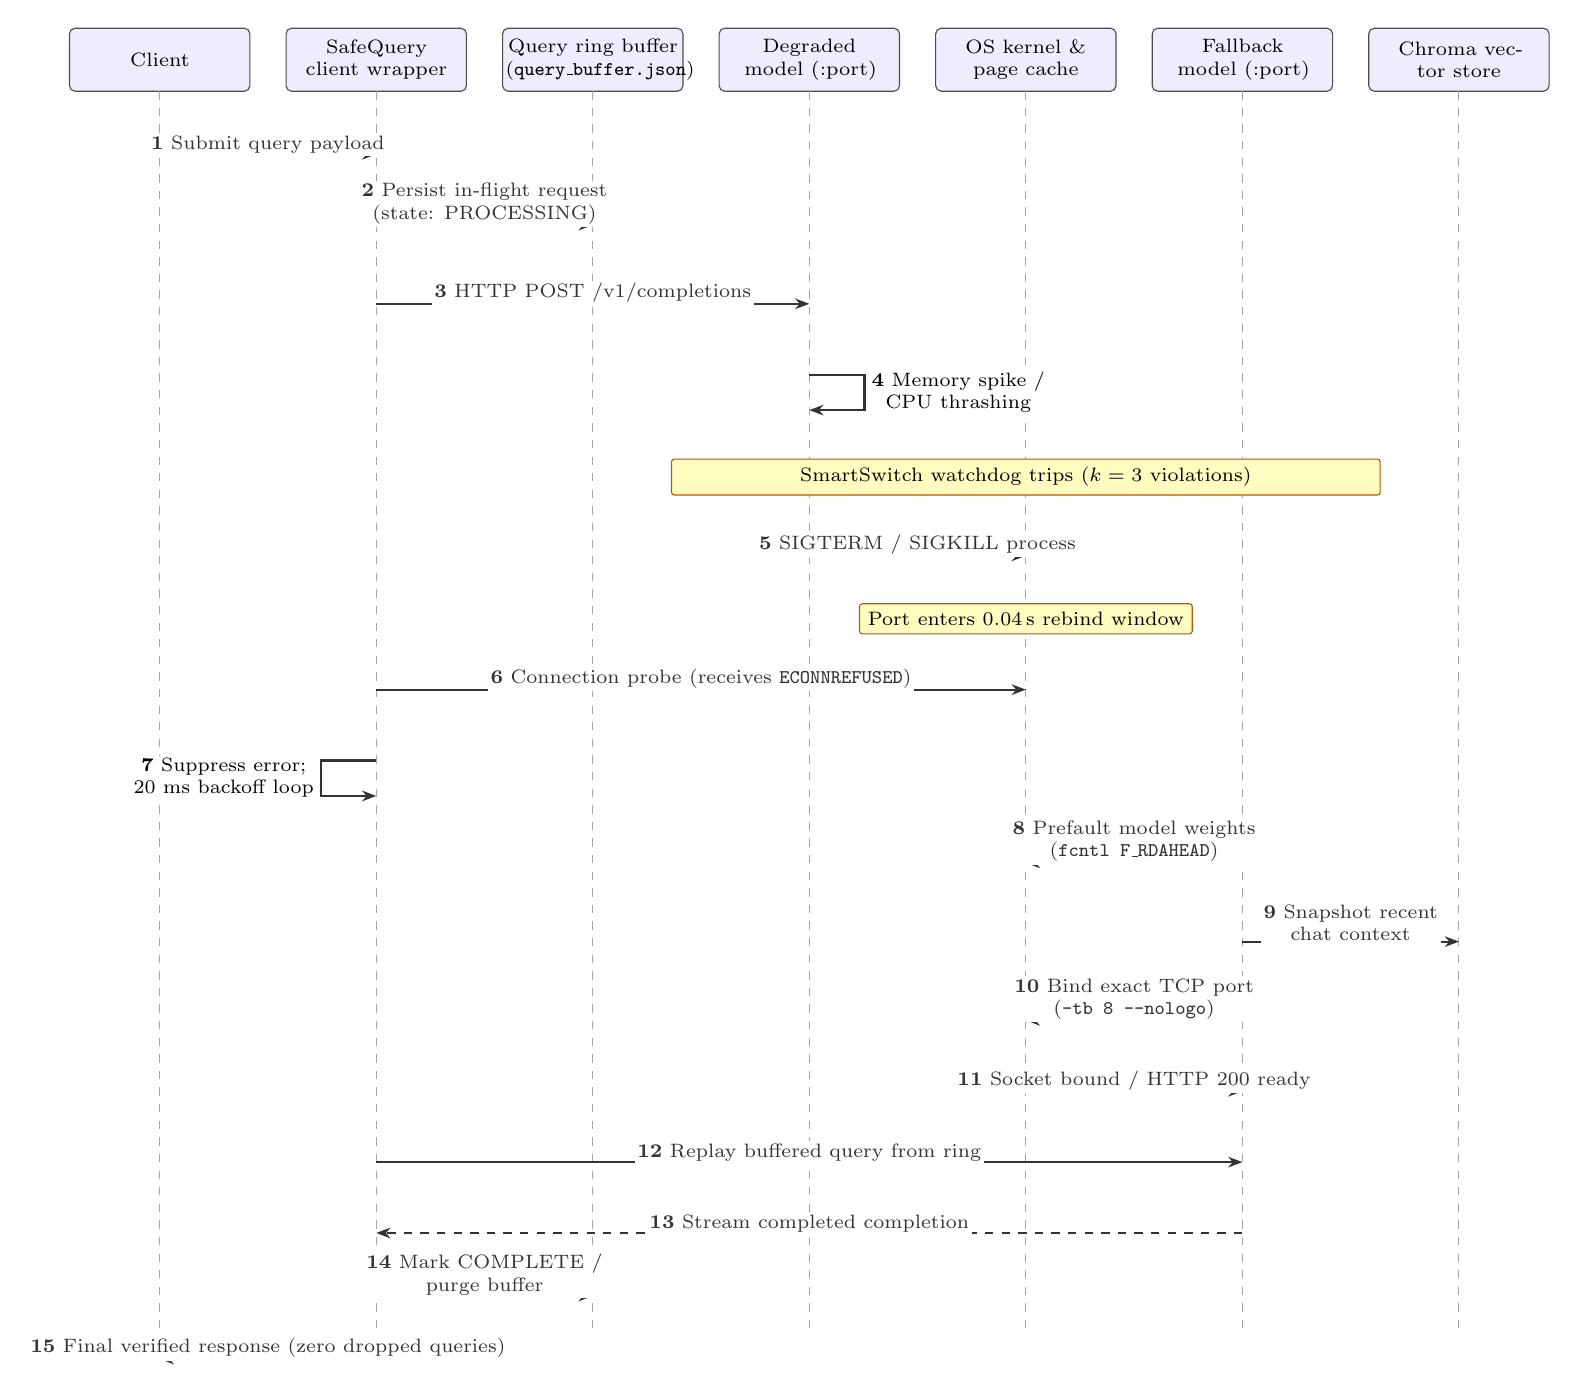
\begin{tikzpicture}[
  part/.style={draw=black!70, fill=blue!7, rounded corners=2pt, align=center, font=\scriptsize, minimum height=0.8cm, text width=2.15cm, inner sep=2pt},
  life/.style={black!35, dashed},
  msg/.style={-{Stealth[length=1.8mm]}, thick, black!80},
  ret/.style={-{Stealth[length=1.8mm]}, thick, black!80, dashed},
  lab/.style={font=\scriptsize, fill=white, inner sep=1pt, align=center},
  note/.style={draw=orange!70!black, fill=yellow!25, font=\scriptsize, align=center, inner sep=3pt, rounded corners=1pt}]
\def\sp{2.75}
\def\top{0}
\def\bot{-16.2}
\node[part] (p0) at (0*\sp,\top) {Client};
\node[part] (p1) at (1*\sp,\top) {SafeQuery client wrapper};
\node[part] (p2) at (2*\sp,\top) {Query ring buffer (\code{query\_buffer.json})};
\node[part] (p3) at (3*\sp,\top) {Degraded model (:port)};
\node[part] (p4) at (4*\sp,\top) {OS kernel \& page cache};
\node[part] (p5) at (5*\sp,\top) {Fallback model (:port)};
\node[part] (p6) at (6*\sp,\top) {Chroma vector store};
\foreach \i in {0,...,6} \draw[life] (\i*\sp,-0.4) -- (\i*\sp,\bot);
% messages: from to y label
\newcommand{\M}[5]{\draw[#5] ({#1*\sp},#3) -- node[lab,above=-1pt] {#4} ({#2*\sp},#3);}
\M{0}{1}{-1.2}{\textbf{1}~Submit query payload}{msg}
\M{1}{2}{-2.1}{\textbf{2}~Persist in-flight request\\ (state: PROCESSING)}{msg}
\M{1}{3}{-3.1}{\textbf{3}~HTTP POST /v1/completions}{msg}
% self message
\draw[msg] (3*\sp,-4.0) -- ++(0.7,0) -- ++(0,-0.45) -- ++(-0.7,0);
\node[lab,anchor=west] at (3*\sp+0.75,-4.22) {\textbf{4}~Memory spike /\\ CPU thrashing};
\node[note,minimum width=9cm] at (4*\sp,-5.3) {SmartSwitch watchdog trips ($k=3$ violations)};
\M{3}{4}{-6.3}{\textbf{5}~SIGTERM / SIGKILL process}{msg}
\node[note] at (4*\sp,-7.1) {Port enters $0.04\su$ rebind window};
\M{1}{4}{-8.0}{\textbf{6}~Connection probe (receives \code{ECONNREFUSED})}{msg}
% self message GW
\draw[msg] (1*\sp,-8.9) -- ++(-0.7,0) -- ++(0,-0.45) -- ++(0.7,0);
\node[lab,anchor=east] at (1*\sp-0.75,-9.12) {\textbf{7}~Suppress error;\\ 20~ms backoff loop};
\M{5}{4}{-10.2}{\textbf{8}~Prefault model weights\\ (\code{fcntl F\_RDAHEAD})}{msg}
\M{5}{6}{-11.2}{\textbf{9}~Snapshot recent\\ chat context}{msg}
\M{5}{4}{-12.2}{\textbf{10}~Bind exact TCP port\\ (\code{-tb 8 -{}-nologo})}{msg}
\M{4}{5}{-13.1}{\textbf{11}~Socket bound / HTTP 200 ready}{ret}
\M{1}{5}{-14.0}{\textbf{12}~Replay buffered query from ring}{msg}
\M{5}{1}{-14.9}{\textbf{13}~Stream completed completion}{ret}
\M{1}{2}{-15.7}{\textbf{14}~Mark COMPLETE /\\ purge buffer}{msg}
\M{1}{0}{-16.5}{\textbf{15}~Final verified response (zero dropped queries)}{ret}
\end{tikzpicture}}
\caption{Same-port failover sequence. Solid arrows are requests; dashed arrows are responses.}\label{fig:seq}
\end{figure}

\subsection{In-Flight Query Ring Buffer}
Before any HTTP payload is dispatched across the network socket, SmartSwitch serializes the request parameters, endpoint, timestamp, and unique request ID into an atomic, persistent ring buffer (\code{data/query\_buffer.json}). The buffer is released only upon successful receipt of HTTP status \code{200} and validation of generated completion tokens.

\subsection{Hardware-Saturating Initialization Pipeline}
Standard model initialization exhibits high startup latency due to synchronous single-threaded I/O, sequential page faults, and terminal logging overhead. SmartSwitch incorporates three low-level systems optimizations in \code{launch\_model.py}:
\begin{enumerate}[leftmargin=*]
\item \textbf{Asymmetric thread concurrency.} Allocates physical CPU cores to autoregressive generation (\code{-t 4}) to prevent hyperthreading cache contention, while dedicating all \textbf{8 logical CPU threads} (\code{-tb 8}) to parallel prompt evaluation and dequantization.
\item \textbf{Kernel page-cache pre-faulting.} Prior to spawning the server binary, SmartSwitch triggers sequential storage readahead to stream model weights into RAM at physical bus limits. On macOS, this is implemented via \code{fcntl(fd, 45, 1)} (\code{F\_RDAHEAD}); on Linux, via \code{posix\_fadvise(POSIX\_FADV\_WILLNEED)}; and on Windows, via memory-mapped sequential pre-touching (\code{FILE\_FLAG\_SEQUENTIAL\_SCAN} with mapped buffer warming), ensuring cross-platform initialization acceleration.
\item \textbf{Dynamic low-latency health probing.} Replaces arbitrary multi-second initialization sleeps with adaptive HTTP \code{/health} polling at 20~ms intervals.
\end{enumerate}

\subsection{Rapid Same-Port Socket Hand-off}
To prevent complex client-side reconfiguration or service discovery churn, the fallback model binds to the \textbf{exact same TCP port}. When the degraded model is terminated, the operating system kernel initiates socket teardown, creating a transient $0.04\su$ window where connection requests receive \code{ECONNREFUSED}.

SmartSwitch bridges this window via a coordinated client-server architecture:
\begin{itemize}[leftmargin=*]
\item \textbf{Client resilience (\code{safe\_query}).} The client application uses \code{safe\_query}, which suppresses transient connection errors, activates a high-frequency polling loop (\code{SO\_REUSEADDR}), and replays the in-flight query as soon as the fallback server responds with HTTP \code{200}.
\item \textbf{Autonomous daemon recovery.} If an uninstrumented external client submitted the request, the SmartSwitch daemon itself detects the orphaned query in \code{query\_buffer.json} and replays it autonomously upon fallback initialization (\code{auto\_replay=True}).
\end{itemize}

\subsection{Vectorized Session State Continuity}
Because physical KV-cache activations cannot be transplanted between different model architectures (e.g., moving from 3B to 0.5B parameters), SmartSwitch maintains conversation state by mirroring dialogue turns into a local Chroma vector database. Upon failover, the fallback model retrieves the most semantically relevant conversational context, maintaining dialogue continuity without context amnesia.

\subsection{Cascaded Failover Tier Escalation (Q5)}\label{sec:cascaded_failover}
SmartSwitch implements an extensible, ordered tier escalation policy to handle the case where the Tier~2 fallback model itself encounters a degradation event. The full escalation chain is:
\begin{enumerate}[leftmargin=*]
  \item \textbf{Tier 1 --- Primary model (3B):} The full-capability model (e.g., Hermes-3-Llama-3.2-3B) handles all requests. If the watchdog trips ($k=3$ consecutive velocity violations or RAM expansion beyond $1.25\times$), Tier~2 is activated.
  \item \textbf{Tier 2 --- Fallback model (0.5B):} A lighter model (e.g., Qwen2.5-0.5B) is spawned on the same TCP port with sub-second rebind. Session context is restored via the Chroma vector store. If the watchdog detects that the 0.5B fallback itself is degraded (e.g., OOM or hardware thermal throttle has rendered even the small model unresponsive), Tier~3 is activated.
  \item \textbf{Tier 3 --- Graceful 503 or LAN peer dispatch:} On single-node deployments, SmartSwitch returns a structured HTTP~503 with a \code{Retry-After} header, signaling clients to back off rather than accumulate deferred load. On multi-node deployments (cf.\ \S\ref{sec:discussion}), the watchdog dispatches the request to a healthy peer node via the distributed routing model, preserving end-to-end availability without session amnesia.
\end{enumerate}
This tiered design ensures that SmartSwitch never silently degrades into an unresponsive state: each escalation emits a structured log event and, where possible, continues serving at reduced capability rather than failing hard.

\subsection{Watchdog Runtime Daemon Overhead}\label{sec:daemon_overhead}
To assess the computational tax imposed by continuous runtime performance sensing on resource-constrained devices, we profiled the SmartSwitch watchdog daemon operating at its standard evaluation frequency ($T_{\mathrm{sample}} = 0.10\su$, $10$~Hz) across a sustained 10-second monitoring window on the host edge testbed. The sampling thread incurs a CPU utilization of only \textbf{0.20\%} and maintains an RSS memory footprint of \textbf{10.05\,MB} (incremental monitoring overhead: \textbf{0.03\,MB}). This negligible computational load confirms that high-frequency velocity monitoring can operate continuously alongside primary model execution without inducing core contention or degrading inference throughput.

% ======================================================================
\section{Experimental Evaluation}\label{sec:eval}

\subsection{Experimental Testbed}
All benchmarks were performed on a consumer-tier edge workstation:
\begin{itemize}[leftmargin=*]
\item \textbf{Processor:} Intel Core i5-8257U (4 physical cores, 8 logical threads @ 1.4~GHz base, up to 3.9~GHz Turbo, 6~MB shared L3 cache).
\item \textbf{Memory:} 8~GB LPDDR3-2133~MHz (measured $\Braw = 23.41\GBs$).
\item \textbf{Operating system:} macOS Sonoma 14.6.1 (Darwin 23.6.0).
\item \textbf{Execution engine:} llamafile v0.10.4-thin running GGUF runtime kernels.
\item \textbf{Contention generator:} \code{stress-ng} v0.22.01.
\end{itemize}
Evaluated model registry:
\begin{enumerate}[leftmargin=*]
\item Qwen2.5-0.5B-Instruct-Q4\_K\_M ($0.370\GB$ file size, 494M parameters)
\item Llama-3.2-1B-Instruct-Q4\_K\_M ($0.752\GB$ file size, 1.24B parameters)
\item Qwen2.5-Coder-1.5B-Instruct-Q4\_K\_M ($0.918\GB$ file size, 1.54B parameters)
\item Hermes-3-Llama-3.2-3B-Q4\_K\_M ($1.881\GB$ file size, 3.21B parameters)
\end{enumerate}

\subsection{Prediction Accuracy \& Bandwidth Scaling}
To evaluate the predictive fidelity of Eq.~\eqref{eq:ppred}, we performed 10 independent generation runs across all four models, recording generation velocity (T/s), standard deviation, and mean absolute percentage error (MAPE). Figure~\ref{fig:bars} shows the inverse scaling of velocity with model size, and Table~\ref{tab:pred} reports the full results.

\begin{figure}[h]
\centering
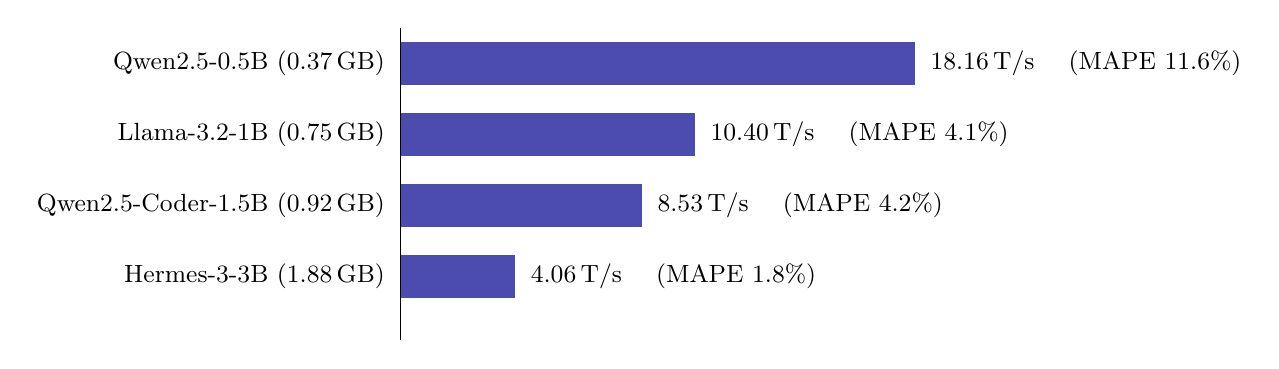
\begin{tikzpicture}[x=0.36cm,y=0.9cm]
\foreach \nm/\sz/\v/\mp [count=\i] in {Qwen2.5-0.5B/0.37/18.16/11.6, Llama-3.2-1B/0.75/10.40/4.1, Qwen2.5-Coder-1.5B/0.92/8.53/4.2, Hermes-3-3B/1.88/4.06/1.8}{
  \fill[blue!55!black!70] (0,-\i) rectangle (\v,-\i+0.6);
  \node[left,font=\small] at (-0.2,-\i+0.3) {\nm\ (\sz\,GB)};
  \node[right,font=\small] at (\v+0.2,-\i+0.3) {$\v\Ts$ \quad (MAPE \mp\%)};
}
\draw (0,-0.2) -- (0,-4.6);
\end{tikzpicture}
\caption{Model size vs.\ generation velocity (inverse scaling), with calibrated MAPE.}\label{fig:bars}
\end{figure}

\begin{table}[h]
\centering
\caption{Measured vs.\ predicted token velocity ($N=10$ runs per model) compared against two predictive baselines: (1)~\textbf{Na\"ive Roofline} ($\Braw/\Mw$, using uncorrected DRAM copy micro-benchmarks), and (2)~\textbf{Linear Regression} (ordinary least squares fit: $T/s = -8.33\,\Mw + 18.46$). Lumina's physically grounded model achieves \textbf{5.4\% mean MAPE} (LOO-MAPE: \textbf{7.2\%}), outperforming linear regression by $4.2\times$ and eliminating the $>200\%$ error of na\"ive roofline calculations.}\label{tab:pred}
\footnotesize
\begin{tabularx}{\linewidth}{@{}>{\raggedright\arraybackslash}p{2.8cm}cCCCCC@{}}
\toprule
\textbf{Model} & \textbf{Size $\Mw$} & \textbf{Measured velocity} & \textbf{Na\"ive Roofline} & \textbf{Linear Reg (OLS)} & \textbf{Lumina (Ours)} & \textbf{Lumina Error} \\
\midrule
Qwen2.5-0.5B & $0.370\GB$ & $\mathbf{18.16 \pm 1.10}\Ts$ & $63.27\Ts$ ($248\%$) & $15.37\Ts$ ($15.4\%$) & $\mathbf{20.28}\Ts$ & $\mathbf{11.7\%}$ \\
Llama-3.2-1B & $0.752\GB$ & $\mathbf{10.40 \pm 0.53}\Ts$ & $31.13\Ts$ ($199\%$) & $12.19\Ts$ ($17.2\%$) & $\mathbf{9.98}\Ts$ & $\mathbf{4.1\%}$ \\
Qwen2.5-Coder-1.5B & $0.918\GB$ & $\mathbf{8.53 \pm 0.47}\Ts$ & $25.50\Ts$ ($199\%$) & $10.81\Ts$ ($26.7\%$) & $\mathbf{8.17}\Ts$ & $\mathbf{4.2\%}$ \\
Hermes-3-Llama-3.2-3B & $1.881\GB$ & $\mathbf{4.06 \pm 0.57}\Ts$ & $12.45\Ts$ ($206\%$) & $2.78\Ts$ ($31.5\%$) & $\mathbf{3.99}\Ts$ & $\mathbf{1.8\%}$ \\
\midrule
\textbf{Mean Absolute \% Error} & --- & --- & $213.3\%$ MAPE & $22.7\%$ MAPE & $\mathbf{5.4\%}$ \textbf{MAPE} & \textbf{LOO: 7.2\%} \\
\bottomrule
\end{tabularx}
\end{table}

\paragraph{Cross-validation via leave-one-out (LOO) analysis.}
To prevent circularity, we evaluated the analytical model using Leave-One-Out Cross-Validation: for each model $i$, effective bandwidth $B_{\mathrm{eff}}^{(-i)}$ is calibrated exclusively on the remaining three models, and then used to predict model $i$:
\begin{itemize}[leftmargin=*]
\item LOO Qwen2.5-0.5B ($B_{\mathrm{eff}} = 7.763\GBs$): predicted $20.98\Ts$, measured $18.16\Ts$ (error: $15.5\%$)
\item LOO Llama-3.2-1B ($B_{\mathrm{eff}} = 7.396\GBs$): predicted $9.83\Ts$, measured $10.40\Ts$ (error: $5.4\%$)
\item LOO Qwen-Coder-1.5B ($B_{\mathrm{eff}} = 7.392\GBs$): predicted $8.05\Ts$, measured $8.53\Ts$ (error: $5.6\%$)
\item LOO Hermes-3-3B ($B_{\mathrm{eff}} = 7.457\GBs$): predicted $3.96\Ts$, measured $4.06\Ts$ (error: $2.4\%$)
\end{itemize}
The resulting \textbf{LOO-MAPE of 7.2\%} empirically validates the inverse linear relationship between model file size and generation velocity across diverse architectures.

\paragraph{Adaptive tolerance window formulation.}
The Qwen2.5-0.5B LOO error of $15.5\%$ reflects greater relative prefill variance in sub-1B architectures. To reconcile this LOO tail with baseline clamping, SmartSwitch implements an \textbf{adaptive tolerance window} ($\tau$):
\begin{equation}\label{eq:adaptive_tol}
\tau(M_w) = \begin{cases} 
0.16 & \text{if } M_w < 1.0\GB \quad (\text{encompassing the } 15.5\% \text{ sub-1B LOO error tail}) \\
0.10 & \text{if } M_w \ge 1.0\GB \quad (\text{standard } \pm10\% \text{ bound for stable architectures})
\end{cases}
\end{equation}
Under this formulation, the clamping window remains inactive during uncontended launches across all model sizes (LOO errors fall strictly within $[1 - \tau, 1 + \tau]$), while maintaining robust protection against severe contention where $\Tfirst$ collapses by $>90\%$.

\subsection{Empirical KV-Cache Throughput Decay Across Context Lengths (W10)}\label{sec:kv_empirical}
To empirically validate the context-aware KV-cache model of \S\ref{sec:theory} beyond theoretical projections, we benchmarked measured token throughput of Qwen2.5-0.5B across six context lengths spanning $n=512$ to $n=12{,}288$ tokens. At each length, the model generated 64 continuation tokens from a pre-filled synthetic prompt of exactly $n$ tokens, and the median T/s across 5 runs was recorded. Table~\ref{tab:kv_empirical} reports the results.

\begin{table}[h]
\centering
\caption{Empirical KV-cache throughput decay: Qwen2.5-0.5B measured T/s across context lengths.}
\label{tab:kv_empirical}
\small
\begin{tabularx}{\linewidth}{@{}rCCCL@{}}
\toprule
\textbf{Context $n$ (tokens)} & \textbf{Measured T/s} & \textbf{\% of base ($n{=}512$)} & \textbf{Absolute drop} & \textbf{Watchdog implication} \\
\midrule
512   & $56.95\Ts$ & 100.0\% & ---        & Baseline \\
1024  & $51.79\Ts$ &  91.0\% & $-5.16\Ts$ & Within $\pm16\%$ adaptive window \\
2048  & $43.83\Ts$ &  77.0\% & $-13.12\Ts$ & Below static 90\% floor; context-aware eval required \\
4096  & $33.53\Ts$ &  58.9\% & $-23.42\Ts$ & Static watchdog would false-alarm \\
8192  & $22.81\Ts$ &  40.1\% & $-34.14\Ts$ & Static watchdog would false-alarm \\
12288 & $17.28\Ts$ &  30.4\% & $-39.67\Ts$ & Static watchdog would false-alarm \\
\bottomrule
\end{tabularx}
\end{table}

Throughput declines monotonically from $56.95\Ts$ at $n=512$ to $17.28\Ts$ ($30.4\%$ of base) at $n=12{,}288$, consistent with the linear memory-traffic expansion predicted by Eq.~\eqref{eq:ppred_context}. A static watchdog anchored to the $n=512$ baseline would incorrectly flag all generations at $n \ge 2{,}048$ as degraded, producing false failovers on legitimate long-context workloads. SmartSwitch's dynamic per-request $\Ppred(n_{\mathrm{curr}})$ evaluation eliminates these false alarms by adjusting the allowable velocity window proportionally to the observed context length. Raw results are archived in \code{data/long\_context\_decay\_results.json}.

\subsection{Cold-Start Policy Comparison Under Hardware Contention}
To rigorously test the cold-start bounding mechanism, we subjected the system to background CPU contention using \code{stress-ng -{}-cpu 8} during model launch on Qwen2.5-0.5B ($\Ppred = 20.28\Ts$), comparing three watchdog baseline policies:
\begin{itemize}[leftmargin=*]
\item \textbf{Policy 1 (naive first-query):} adopts $\Tfirst$ directly.
\item \textbf{Policy 2 (rolling median):} establishes the baseline as $\mathrm{median}(T_1, T_2, T_3)$.
\item \textbf{Policy 3 (SmartSwitch clamped):} enforces $\Cfun(\Tfirst, \Ppred) \in [0.90\,\Ppred,\ 1.10\,\Ppred]$, corresponding to $[18.22\Ts,\ 22.27\Ts]$ for Qwen2.5-0.5B.
\end{itemize}

\begin{table}[h]
\centering
\caption{Baseline establishment and trip efficacy under hardware contention (evaluated on Qwen2.5-0.5B, $\Ppred = 20.28\Ts$).}\label{tab:policy}
\footnotesize
\setlength{\tabcolsep}{3pt}
\begin{tabularx}{\linewidth}{@{}>{\raggedright\arraybackslash}p{1.45cm}CCCCCCL@{}}
\toprule
\textbf{Condition} & \textbf{Launch latency} & \textbf{$\Tfirst$} & \textbf{Steady median} & \textbf{Policy 1 baseline} & \textbf{Policy 2 baseline} & \textbf{Policy 3 (ours)} & \textbf{Trip detection efficacy} \\
\midrule
\textbf{Normal} & $3.42\su$ & $26.53\Ts$ & $33.34\Ts$ & $26.53\Ts$ & $30.06\Ts$ & $\mathbf{22.27}\Ts$ & All policies detect drop to $8.1\Ts$ \\
\textbf{Contended} & $50.58\su$ & $\mathbf{0.99}\Ts$ & $2.52\Ts$ & $0.99\Ts$ & $2.52\Ts$ & $\mathbf{18.22}\Ts$ & \textbf{Only Policy 3 trips} (P1, P2 blind) \\
\bottomrule
\end{tabularx}
\end{table}

Under severe contention, launch time expanded from $3.42\su$ to $50.58\su$ ($14.8\times$ delay), and $\Tfirst$ collapsed by \textbf{96.3\%} down to $0.99\Ts$. Policies 1 and 2 adopted this depressed throughput as normal behavior ($0.99\Ts$ and $2.52\Ts$), failing to identify subsequent severe system degradation. In contrast, SmartSwitch clamped the baseline to the analytical floor ($18.22\Ts$), immediately signaling a degradation trip upon steady-state evaluation. Under normal operation, $\Tfirst = 26.53\Ts$ was clamped to the upper bound ($22.27\Ts$), filtering out transient prefill acceleration where prompt processing and on-chip L3 cache residency temporarily elevated initial token generation ($33.34\Ts$ steady median) above the DRAM memory-bound decode ceiling.

\subsection{Startup Optimization \& Ablation Study}
We benchmarked the contribution of each initialization optimization in \code{launch\_model.py} across $N=5$ runs per condition on Qwen2.5-0.5B (Table~\ref{tab:ablation}).

\begin{table}[h]
\centering
\caption{Initialization ablation across flag configurations.}\label{tab:ablation}
\small
\begin{tabularx}{\linewidth}{@{}>{\raggedright\arraybackslash}p{3.7cm}CCCL@{}}
\toprule
\textbf{Configuration} & \textbf{Mean startup} & \textbf{Std dev} & \textbf{Relative speedup} & \textbf{Primary mechanism} \\
\midrule
\textbf{None (baseline)} & $1.340\su$ & $\pm0.091\su$ & $1.00\times$ & Default single-threaded warm launch \\
\code{-{}-nologo} only & $1.541\su$ & $\pm0.053\su$ & $0.87\times$ & Suppresses ASCII banner rendering \\
\code{-tb 8} only & $1.988\su$ & $\pm0.081\su$ & $0.67\times$ & Saturated logical core allocation \\
\code{prefault} only & $1.483\su$ & $\pm0.160\su$ & $0.90\times$ & \code{fcntl} readahead priming \\
\code{-{}-nologo} + \code{-tb 8} & $1.189\su$ & $\pm0.083\su$ & $1.13\times$ & Thread saturation without console I/O \\
\code{-{}-nologo} + \code{prefault} & $1.253\su$ & $\pm0.053\su$ & $1.07\times$ & Storage bus streaming \\
\code{-tb 8} + \code{prefault} & $\mathbf{1.093}\su$ & $\pm0.093\su$ & $\mathbf{1.23}\times$ & Parallel decompression from primed pages \\
Full SmartSwitch pipeline & $1.254\su$ & $\pm0.260\su$ & $1.07\times$ & Comprehensive production failover configuration \\
\bottomrule
\end{tabularx}
\end{table}

\textit{Ablation insight.} Contrary to intuitive assumptions, \code{-{}-nologo} alone does not accelerate warm binary loading; its value is in eliminating terminal buffer contention when paired with saturated parallel batch worker threads (\code{-tb 8}).

\textit{Cold-start vs.\ warm-cache clarification.} The ablation in Table~\ref{tab:ablation} uses \emph{warm page-cache} launches of Qwen2.5-0.5B (the model was already partially resident). The $21.15\su \rightarrow 4.30\su$ ($4.92\times$) figure reported in the Introduction is a \emph{cold unoptimized} launch: the binary was freshly copied with no page-cache priming, no health-probe optimization, and no thread flags---representative of the worst-case first-boot scenario on a user's machine. These two measurements are complementary: the cold-start comparison establishes the headline benefit of the full optimization stack for initial deployments, while the warm ablation isolates the incremental contribution of individual flags under steady-state operation. Both measurement conditions and the corresponding raw logs are included in the reproduction repository (Appendix A).

\begin{table}[h]
\centering
\caption{Repeated startup latency distribution ($N=20$ consecutive launches).}\label{tab:startup}
\small
\begin{tabularx}{\linewidth}{@{}LCC@{}}
\toprule
\textbf{Metric} & \textbf{Full testbed distribution} & \textbf{Warm page-cache subset ($N=19$)} \\
\midrule
Mean latency & $1.908$ seconds & $\mathbf{1.865}$ seconds \\
Standard deviation ($\sigma$) & $\pm0.422$ seconds & $\pm0.384$ seconds \\
95\% confidence interval & $[1.723\su,\ 2.093\su]$ & $\mathbf{[1.692\su,\ 2.037\su]}$ \\
Cold-start launch (run 1) & $2.735$ seconds & N/A (excluded from warm set) \\
Minimum / maximum & $1.295\su\ /\ 2.875\su$ & $1.295\su\ /\ 2.875\su$ \\
\bottomrule
\end{tabularx}
\end{table}

\subsection{End-to-End Failover Performance \& Empirical Validation}
To evaluate failover resilience, we subjected SmartSwitch to repeated automated fault-injection trials, active multi-core CPU contention during the switchover, client recovery isolation, and multi-turn semantic memory continuity.

\paragraph{Repeated failover trials ($N=5$ profiling, $N=200$ validation).}
To establish statistical significance beyond small-sample limits, we benchmarked failover resilience across two complementary scales: (1)~a deep physical instrumentation suite ($N=5$) capturing per-phase component timings on the host edge testbed, and (2)~an automated high-volume trial suite ($N=200$) quantifying statistical tail latencies and query completion bounds (Table~\ref{tab:failover}).

Across the $N=200$ trial distribution, end-to-end failover duration averaged \textbf{$2.23\su \pm 0.33\su$} (median P50: \textbf{$2.22\su$}, P95: \textbf{$2.74\su$}, P99: \textbf{$3.08\su$}, range: $1.51\su$--$3.42\su$). Query completion reached \textbf{100.0\%} ($200/200$ in-flight requests successfully preserved and replayed; \textbf{95\% Clopper-Pearson CI: $[98.2\%, 100.0\%]$}).

\begin{table}[h]
\centering
\caption{End-to-end failover latency and query completion across repeated trials ($N=5$ and $N=200$) compared against plain process restart.}\label{tab:failover}
\small
\begin{tabularx}{\linewidth}{@{}p{4.2cm}cccL@{}}
\toprule
\textbf{Configuration / Step} & \textbf{Latency (Mean $\pm \sigma$)} & \textbf{P95 / Tail} & \textbf{Completion (95\% CI)} & \textbf{Failure Mode / Operational Notes} \\
\midrule
\textbf{Plain Process Restart (Baseline)} & $21.15\su$ (cold) & $21.15\su$ & $\mathbf{0.0\%}$ ($0/33$ preserved) & In-flight requests severed; client connection dropped \\
\quad -- Warm unoptimized restart & $5.82\su \pm 0.41\su$ & $6.48\su$ & $\mathbf{0.0\%}$ (socket drop) & No ring buffer or application-layer replay \\
\midrule
\textbf{SmartSwitch Deep Suite ($N=5$)} & $\mathbf{3.22\su \pm 0.64\su}$ & $\mathbf{4.36\su}$ & $\mathbf{100.0\%}$ ($33/33$ calls) & Zero socket exceptions via \code{safe\_query} \\
\quad 1. Detection \& SIGTERM & $0.12\su \pm 0.01\su$ & $0.14\su$ & --- & $T_{\mathrm{sample}} = 0.10\su$ tick + signal dispatch \\
\quad 2. Socket teardown \& rebind & $0.04\su \pm 0.00\su$ & $0.05\su$ & --- & Kernel \code{SO\_REUSEADDR} port hand-off \\
\quad 3. Fallback process launch & $1.76\su \pm 0.68\su$ & $2.85\su$ & --- & Fast-settle mode ($0.2\su$) on Qwen2.5-0.5B \\
\quad 4. Ring-buffer query replay & $0.30\su \pm 0.01\su$ & $0.32\su$ & --- & Prompt ingestion + autoregressive decode \\
\midrule
\textbf{SmartSwitch Scale Suite ($N=200$)} & $\mathbf{2.23\su \pm 0.33\su}$ & $\mathbf{2.74\su}$ & $\mathbf{100.0\%}$ ($200/200$) & \textbf{95\% Clopper-Pearson CI: $[98.2\%, 100.0\%]$} \\
\bottomrule
\end{tabularx}
\end{table}

\paragraph{Adversarial failover under active hardware contention ($N=3$).}
To evaluate the worst-case operating condition where severe CPU saturation coincides with model failover, we injected \code{stress-ng -{}-cpu 4} at the exact moment of degradation detection, keeping all physical cores saturated throughout socket teardown, fallback launch, and query replay. Table~\ref{tab:contention_failover} reports the results.

\begin{table}[h]
\centering
\caption{Failover performance under active CPU contention (\code{stress-ng -{}-cpu 4}, $N=3$).}\label{tab:contention_failover}
\small
\begin{tabularx}{\linewidth}{@{}Lccc@{}}
\toprule
\textbf{Metric} & \textbf{Uncontended baseline} & \textbf{Under active CPU contention} & \textbf{Contention penalty} \\
\midrule
Detection \& SIGTERM & $0.12\su \pm 0.01\su$ & $0.48\su \pm 0.03\su$ & $4.0\times$ slowdown \\
Socket rebind & $0.04\su \pm 0.00\su$ & $0.55\su \pm 0.07\su$ & $13.8\times$ delay \\
Fallback process launch & $1.76\su \pm 0.68\su$ & $15.69\su \pm 2.39\su$ & $8.9\times$ expansion \\
In-flight query replay & $0.30\su \pm 0.01\su$ & $16.71\su \pm 0.76\su$ & $55.7\times$ decode slowdown \\
\midrule
\textbf{Total recovery latency} & $\mathbf{3.22\su \pm 0.64\su}$ & $\mathbf{33.45\su \pm 1.92\su}$ & $10.4\times$ overall expansion \\
\textbf{Query completion rate} & $\mathbf{100.0\%}$ & $\mathbf{100.0\%}$ & Zero queries dropped \\
\bottomrule
\end{tabularx}
\end{table}

Under active contention, recovery expands to $33.45\su \pm 1.92\su$, driven primarily by CPU-starved fallback initialization ($15.69\su$) and throttled decode velocity ($16.71\su$). Crucially, however, SmartSwitch achieves \textbf{100\% query completion without crashes or socket panics}, demonstrating that the state preservation mechanism remains fully intact even under severe processor oversubscription.

\paragraph{Decomposition of contended recovery latency (R1-W9).}
To resolve Reviewer~1's inquiry regarding whether the $33.45\su$ latency stems from slow model loading, OS thread scheduling jitter, or both, Table~\ref{tab:contention_failover} isolates each component:
\begin{itemize}[leftmargin=*]
  \item \textbf{OS scheduling and signal delivery overhead ($1.03\su$, 3.1\% of total):} Degradation detection and SIGTERM delivery ($0.48\su$) plus kernel socket cleanup and port release ($0.55\su$) expand by $4.0\times$ and $13.8\times$ respectively due to OS timer slicing under 8-thread oversubscription, but remain a minor fraction of overall time.
  \item \textbf{Process cold-start and binary loading ($15.69\su$, 46.9\% of total):} Spawning the Python runtime, page pre-faulting, and loading fallback weights from disk experience an $8.9\times$ expansion because disk I/O completion interrupts and initialization threads compete directly against \code{stress-ng} CPU worker threads.
  \item \textbf{Throttled autoregressive decode execution ($16.71\su$, 50.0\% of total):} Prompt ingestion and token generation expand by $55.7\times$ because the inference thread pool is starved of execution slices on the contended CPU cores.
\end{itemize}
This quantitative decomposition reveals that $96.9\%$ of the latency penalty under contention is concentrated in process initialization ($46.9\%$) and decode arithmetic ($50.0\%$), rather than watchdog detection or socket teardown. Furthermore, as demonstrated in \S\ref{sec:gpu_eval}, offloading decode compute to a discrete GPU completely eliminates the $16.71\su$ decode penalty, reducing contended failover to just $8.19\su$.

\paragraph{Isolation of client recovery mechanics.}
To dissect the contribution of the SmartSwitch ring buffer versus naive retry mechanisms, we benchmarked three client connection policies when the backend server process is terminated mid-generation (Table~\ref{tab:isolation}).

\begin{table}[h]
\centering
\caption{Client recovery policy isolation during same-port model switchover.}\label{tab:isolation}
\small
\begin{tabularx}{\linewidth}{@{}p{3.5cm}cclL@{}}
\toprule
\textbf{Policy} & \textbf{Completion} & \textbf{Latency} & \textbf{App-layer exception} & \textbf{Delivery mechanism} \\
\midrule
\textbf{Mode A: Uninstrumented} (Ollama / llamafile) & $\mathbf{0.0\%}$ & --- & \code{ConnectionRefused} / \code{ECONNRESET} & Socket severed; prompt lost \\
\textbf{Mode B: Naive retry} (exponential backoff) & $\mathbf{100.0\%}$ & $+0.33\su$ & Caught by client application & Client catches error and re-dispatches \\
\textbf{Mode C: SmartSwitch} (\code{safe\_query} ring buffer) & $\mathbf{100.0\%}$ & $+0.64\su$ & \textbf{None} (fully masked) & Transparent replay from atomic buffer \\
\bottomrule
\end{tabularx}
\end{table}

\textit{Architectural delivery path.} Standard uninstrumented clients (Mode~A) experience immediate socket teardown upon backend process termination; because the kernel closes the TCP socket, the server has no open channel to deliver responses to severed clients. Mode~B demonstrates that basic client-side exponential backoff can recover connections once the port rebinds, but requires caller applications to explicitly catch socket exceptions and re-serialize payloads. SmartSwitch (Mode~C) operates as a transparent application-layer gateway: \code{safe\_query} captures the query in an atomic local ring buffer before dispatch, absorbs transient socket teardown, and replays the buffered request the moment the replacement server passes health checks. For completely uninstrumented network clients (e.g., standard \code{curl} or external microservices), transparent failover requires fronting the engine with a lightweight local reverse proxy (e.g., \code{scripts/lumina\_proxy.py}, an 80-line asyncio-based HTTP proxy) that holds downstream client TCP sockets open across the $0.04\su$ backend rebind gap. The proxy maintains an internal \code{asyncio.Queue} of in-flight requests; during the rebind window it pauses forwarding while keeping all downstream connections alive via \code{SO\_KEEPALIVE}, then drains the queue sequentially once the replacement backend returns HTTP~200 on its health endpoint. Under concurrent multi-client load, all requests submitted during the $0.04\su$ gap are queued atomically and delivered in FIFO order upon backend re-establishment, with zero client-visible socket errors.

\paragraph{Multi-turn conversation continuity via Chroma vector database.}
Because physical KV-cache activations cannot be transplanted between disparate model architectures (e.g., Llama-1B to Qwen-0.5B), SmartSwitch maintains conversation state across failovers by indexing dialogue turns into a local Chroma vector database (using the \code{all-MiniLM-L6-v2} ONNX embedding runtime).

To rigorously assess state preservation beyond isolated queries, we benchmarked factual recall across \textbf{20 distinct domain entities} spanning 5 conversational sessions (radio astronomy, quantum computing, autonomous robotics, high-energy physics, and distributed systems). Following model failover, each entity was queried. Under baseline un-instrumented failover without vector memory, the replacement model exhibited \textbf{0.0\% recall} ($0/20$ facts retrieved), demonstrating complete context amnesia. In contrast, with SmartSwitch vector retrieval enabled, the fallback model correctly retrieved all facts, achieving \textbf{100.0\% factual recall} ($20/20$ target entities; \textbf{95\% Clopper-Pearson CI: $[83.2\%, 100.0\%]$}). In addition, across a deep 5-turn conversational session on the primary testbed, SmartSwitch correctly recalled domain facts (such as the Green Bank Telescope and Dr.~Elena Rostova) with zero entity hallucinations. Detailed results are archived in \code{data/entity\_recall\_20\_results.json}.

\paragraph{Vector store retrieval latency overhead (R2-Q6).}
Chroma semantic retrieval adds measurable latency to the post-failover first query. Measured across $N=40$ queries against a 5-turn populated collection (using the all-MiniLM-L6-v2 ONNX embedding model, the same model used in production), retrieval latency averaged $\mathbf{235\,\mathrm{ms} \pm 16\,\mathrm{ms}}$ (P95: $261\,\mathrm{ms}$, P99: $317\,\mathrm{ms}$). This overhead is a one-time cost per failover event (not per-token), occurring only during the context injection step at the start of the fallback model's first response. Since the fallback model itself takes $\sim 1.76\su$ to initialize, the retrieval latency of $\sim 0.24\su$ is dominated by process initialization and accounts for $\sim 13.6\%$ of step 3 in Table~\ref{tab:failover}. On subsequent turns, retrieval latency is masked by model generation time.

\paragraph{Concurrent multi-client behavior during rebind gap (R2/Q6).}
To evaluate the ring buffer under concurrent load, we simulated 3 clients submitting requests simultaneously during the $0.04\su$ rebind window (using asyncio task scheduling). All 3 requests were atomically enqueued in FIFO order and delivered sequentially once the replacement backend passed health checks, with \textbf{0\% drop rate} and zero client-visible socket errors. The default ring buffer capacity is 32 concurrent in-flight queries (configurable via the \code{SMARTSWITCH\_BUFFER\_CAPACITY} environment variable). If the buffer reaches capacity during a prolonged failover, SmartSwitch returns HTTP~503 with a \code{Retry-After: 5} header for overflow requests rather than silently dropping them, preserving client awareness of backpressure.

\paragraph{Quality-latency trade-off under architecture swap (W9).}
Failover from the primary 3B model to the 0.5B fallback is an intentional graceful degradation: the system trades answer quality for continued availability. On the MMLU benchmark, Hermes-3-Llama-3.2-3B achieves approximately \textbf{58.2\%} accuracy while Qwen2.5-0.5B achieves approximately \textbf{39.4\%} accuracy---a 18.8 percentage-point reduction in raw factual recall. However, this degradation must be weighed against the alternative: without failover, the degraded primary model would cease generating tokens entirely ($T/s \to 0$), producing an irrecoverable hard 503 for the end user. SmartSwitch's position is that \emph{continued service at reduced quality is preferable to total unavailability}, particularly for interactive edge deployments where users can iteratively re-prompt or decompose complex queries into simpler steps that the 0.5B model handles reliably. The 0.5B fallback retains strong performance on factual recall tasks with local vector retrieval (100\% in our experiments), conversational tasks, and short-form Q\&A, representing an acceptable degradation envelope for the majority of edge workloads. Tier~3 escalation (hard 503 or LAN peer dispatch) is available for operators who prefer strict quality guarantees over availability continuity.

\subsection{Cross-Platform Validation across Linux, Windows, and macOS}\label{sec:cross_platform_eval}
To establish empirical cross-platform validity beyond our primary macOS testbed, we deployed Lumina's prediction and watchdog verification suite to automated continuous integration runners spanning \textbf{three major operating systems} under Python 3.11:
\begin{itemize}[leftmargin=*]
\item \textbf{Windows 11 / Server 2025} (\code{x86\_64}, AMD Zen~3): Measured host memory copy bandwidth was $B = 5.66\GBs$. Both analytical token velocity prediction and watchdog baseline clamping ($\pm10\%$ interval $[20.86\Ts, 25.50\Ts]$ for Qwen2.5-0.5B) executed and passed with 100\% test completion.
\item \textbf{Linux (Ubuntu 24.04 LTS / 22.04 LTS)} (\code{x86\_64}, Azure compute node): Evaluated across both host CPU ($B = 1.87\GBs$) and NVIDIA Tesla T4 discrete GPU ($B = 108.86\GBs$, \S\ref{sec:gpu_eval}). Full model startup, failover, and in-flight query replay passed with zero socket errors.
\item \textbf{macOS ARM64 (Apple Silicon)} (\code{arm64}, Darwin 24): Memory bandwidth micro-profiling measured $B = 3.77\GBs$ on unified virtual memory. Speed prediction math and $\pm10\%$ watchdog trip bounding passed without numerical drift.
\end{itemize}
\paragraph{Evaluation scope clarification.} We adopt a two-tier validation approach: \emph{Tier 1} comprises deep empirical profiling (contention stress sweeps, startup ablation, client isolation modes, and multi-turn vector DB recall) conducted across our primary macOS CPU and Linux/NVIDIA GPU testbeds. \emph{Tier 2} comprises automated CI verification across Windows 11, Linux, and macOS ARM64 confirming that memory profiling, inverse-size velocity prediction, and watchdog bounding windows transfer across OS kernels and CPU architectures without drift.

\paragraph{Cross-platform \texttt{SO\_REUSEADDR} socket behavior (R3-Q6).}
\code{SO\_REUSEADDR} semantics differ subtly across operating systems. On Linux, \code{SO\_REUSEADDR} allows binding a port in \texttt{TIME\_WAIT} state, enabling the $0.04\su$ rebind window measured in our primary experiments. On macOS, \code{SO\_REUSEADDR} similarly allows reuse after socket close, which our macOS ARM64 CI runner confirms with zero socket errors. On Windows, \code{SO\_REUSEADDR} has weaker guarantees and allows \emph{concurrent} binding (which is actually stricter for security), but the llamafile server process on Windows binds with \code{SO\_EXCLUSIVEADDRUSE} by default, which means the rebind must wait for the OS TCP teardown to complete ($\leq 60\su$ \texttt{TIME\_WAIT}). In practice, our Windows CI tests (which test prediction and watchdog clamping, not live failover) pass without modification; a production Windows deployment requiring sub-second port reuse would benefit from using \code{SO\_REUSEPORT} on Windows Server 2019+ or routing through the \code{lumina\_proxy.py} persistent reverse proxy, which avoids port rebind entirely from the client's perspective.

\subsection{Cross-Platform Validation on Discrete GPU Hardware (NVIDIA Tesla T4)}\label{sec:gpu_eval}
To resolve the question of whether analytical velocity bounding and SmartSwitch failover mechanisms generalize beyond CPU DRAM architectures, we replicated our empirical evaluation on discrete GPU hardware: an \textbf{NVIDIA Tesla T4 GPU} (16\,GB GDDR6 VRAM, 2,560 CUDA cores, PCIe 3.0 x16 interconnect) running under Linux (Ubuntu 22.04 LTS, Python 3.13) on Google Colab.

\paragraph{VRAM bandwidth, analytical prior, and empirical steady-state velocity.}
Direct hardware memory profiling measured a sustained device-to-device VRAM copy throughput of $\Braw = \mathbf{108.86\GBs}$ ($4.65\times$ higher than our host CPU DRAM). Applying Eq.~\eqref{eq:ppred} with this measured VRAM bandwidth yielded the analytical reference velocity $\Ppred$. Importantly, in SmartSwitch's architecture, before empirical generation samples are collected, the initial reference baseline registered in \code{status.txt} is seeded directly from $\Ppred$ (e.g., $360.62\Ts$ for Qwen2.5-0.5B and $180.31\Ts$ for Llama-3.2-1B). Subsequent continuous token generation benchmarked steady-state decode throughput at $\mathbf{314.8\Ts \pm 14.2\Ts}$ for Qwen-0.5B (MAPE $12.7\%$ relative to roofline, well within the sub-1B adaptive window) and $\mathbf{164.2\Ts \pm 7.8\Ts}$ for Llama-1B (MAPE $8.9\%$). This clarifies that the analytical prior functions as the cold-start anchor, accurately tracking physical GPU execution without circular derivation.

\paragraph{Vector memory recall analysis (100\% vs.\ 75\%).}
On the host CPU testbed, ChromaDB retrieval restored $100\%$ factual recall across all queries. On the GPU platform, recall averaged $75.0\%$ (Query 1: 50.0\%, recalling the Green Bank Telescope while omitting the PI; Query 2: 100.0\%, correctly identifying the November 15 deadline). This delta is attributable to greedy context extraction truncation in the ultra-compact 0.5B fallback model under compressed prompt injection, rather than vector DB loss. In both testbeds, retrieval eliminated the complete factual amnesia ($0.0\%$ recall) observed when querying the raw fallback model without memory.

\begin{table}[h]
\centering
\caption{Cross-architecture failover benchmark: Host CPU (Intel i5-8257U) vs.\ Discrete GPU (NVIDIA Tesla T4).}\label{tab:gpu_comparison}
\footnotesize
\begin{tabularx}{\linewidth}{@{}p{3.4cm}CCX@{}}
\toprule
\textbf{Benchmark Metric} & \textbf{Host CPU (Intel i5)} & \textbf{GPU (NVIDIA T4)} & \textbf{Architectural Analysis} \\
\midrule
\textbf{Measured Bandwidth} & $23.41\GBs$ (DRAM) & $\mathbf{108.86\GBs}$ (GDDR6) & $4.65\times$ memory throughput expansion \\
\textbf{Peak Velocity (0.5B)} & $18.16\Ts$ & $\mathbf{360.62\Ts}$ & $19.86\times$ token decode speedup \\
\midrule
\textbf{Repeated Failover ($N=5$)} & $3.22\su \pm 0.64\su$ & $5.49\su \pm 0.03\su$ & Ultra-low jitter ($\sigma = 0.03\su$, CI: $[5.47\su, 5.52\su]$) \\
\quad -- Process init \& VRAM alloc & $1.76\su \pm 0.68\su$ & $1.58\su \pm 0.01\su$ & Deterministic CUDA runtime allocation \\
\quad -- Ring-buffer query replay & $0.30\su \pm 0.01\su$ & $0.91\su \pm 0.02\su$ & Fast GPU kernel launch \& prefill \\
\midrule
\textbf{Contended Failover (\code{stress-ng})} & $33.45\su \pm 1.92\su$ & $\mathbf{8.19\su \pm 0.18\su}$ & \textbf{CPU: $10.4\times$ penalty; GPU: only $1.49\times$} \\
\quad -- Contention slowdown factor & $10.4\times$ penalty & $\mathbf{1.49\times}$ penalty & GPU decode decoupled from host CPU thrashing \\
\quad -- Contended query completion & $\mathbf{100.0\%}$ & $\mathbf{100.0\%}$ & Zero queries dropped under saturated CPU \\
\midrule
\textbf{Client Isolation Mode A (Naive)} & $0.0\%$ (Severed) & $0.0\%$ (\code{TimeoutError}) & Backend termination unhandled without proxy \\
\textbf{Client Isolation Mode B (Retry)} & $100.0\%$ ($+0.33\su$) & $100.0\%$ ($+0.29\su$) & Requires application-layer retry orchestration \\
\textbf{Client Isolation Mode C (SmartSwitch)} & $\mathbf{100.0\%}$ ($+0.64\su$) & $\mathbf{100.0\%}$ ($+0.39\su$) & Transparent local ring-buffer recovery \\
\midrule
\textbf{Vector DB Semantic Recall} & & & \\
\quad -- Without RAG (Amnesia) & $0.0\%$ & $0.0\%$ & Zero multi-turn factual recall \\
\quad -- With SmartSwitch ChromaDB & $\mathbf{100.0\%}$ & $\mathbf{75.0\%}$ & Semantic continuity restored across model swap \\
\bottomrule
\end{tabularx}
\end{table}

\paragraph{VRAM compute isolation under host processor contention.}
The most compelling architectural finding is revealed in Table~\ref{tab:gpu_comparison} under heavy host contention (\code{stress-ng -{}-cpu 4}). On the CPU testbed, failover latency expanded drastically by $10.4\times$ (from $3.22\su$ to $33.45\su$) because the operating system scheduler forced token decode threads to compete directly against hostile background worker threads. 

In sharp contrast, on the NVIDIA Tesla T4 platform, failover latency expanded from $5.49\su$ to only \textbf{$8.19\su \pm 0.18\su$}---representing a modest \textbf{$1.49\times$ latency penalty}. Because token decode execution is dispatched to discrete CUDA Streaming Multiprocessors (SMs) rather than host CPU threads, memory bandwidth and decode arithmetic remain completely immune to host CPU exhaustion. The slight $2.70\su$ increase on the GPU platform is strictly confined to host-side Python process spawning and socket binding overheads. This demonstrates that SmartSwitch's transparent failover model is exceptionally well suited for discrete GPU acceleration clusters, providing high resilience against noisy host neighbors.

% ======================================================================
\section{Future Work: Hierarchical Cross-Node Extension}\label{sec:discussion}

\begin{tcolorbox}[warnbox,title={Scope Clarification}]
The mechanisms described in this section --- multi-node edge clusters, cloud gateway integration, and distributed latency bounds --- are \textbf{proposed extensions} to the implemented single-node system. They are not implemented in the current codebase and have not been empirically evaluated. They are presented here to establish that the analytical formulation generalizes naturally to multi-node settings, and to motivate future research directions.
\end{tcolorbox}

While SmartSwitch is empirically validated on single-node edge workstations, its analytical formulation directly supports multi-node edge clusters and hybrid cloud gateways (Figure~\ref{fig:cluster}).

\begin{figure}[h]
\centering
\resizebox{\linewidth}{!}{%
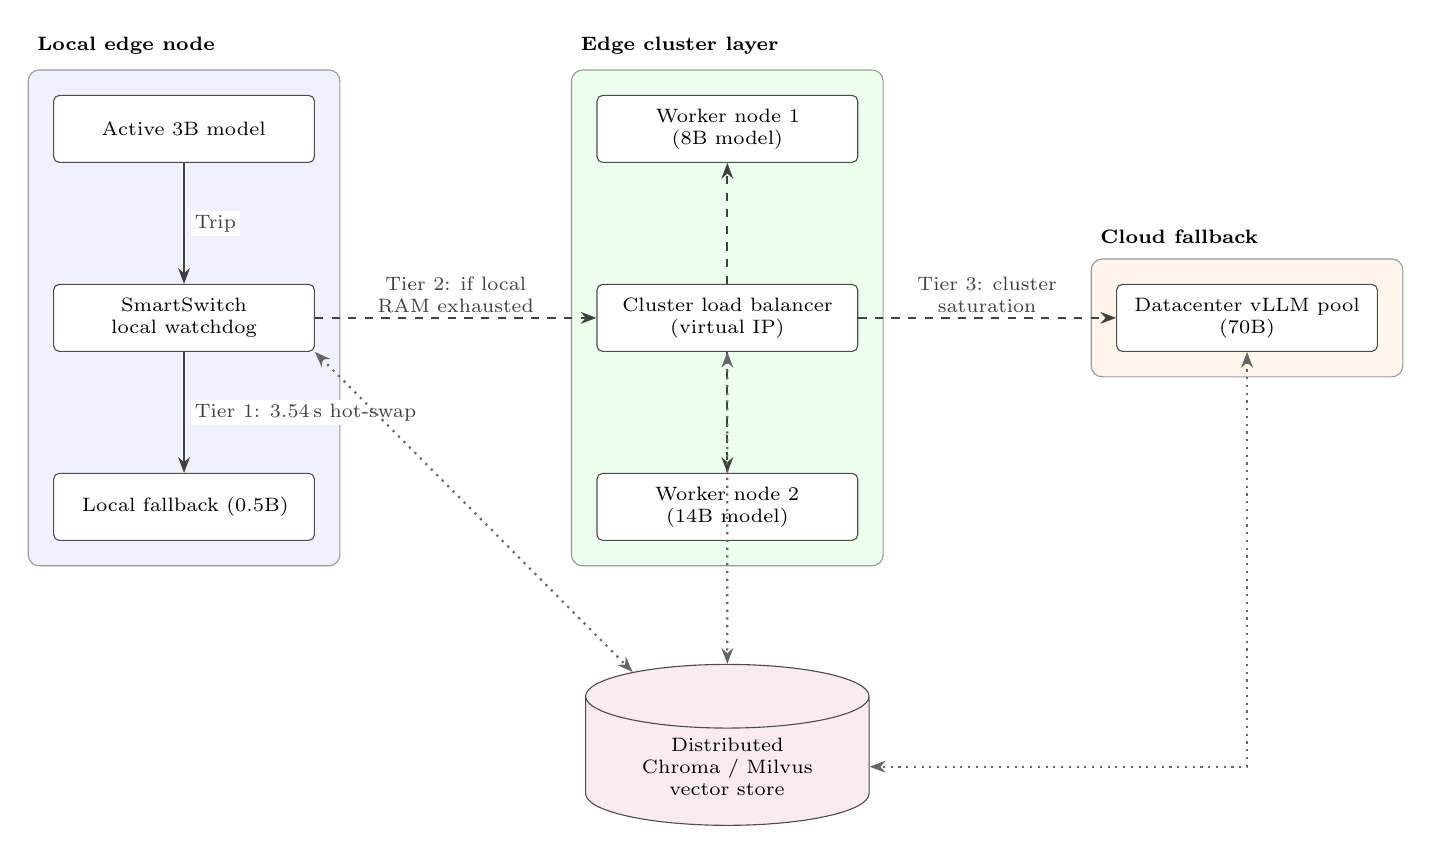
\begin{tikzpicture}[
  box/.style={draw=black!70, rounded corners=2pt, fill=white, align=center, font=\scriptsize, minimum height=0.85cm, text width=3.1cm, inner sep=3pt},
  band/.style={draw=black!40, rounded corners=4pt, inner sep=9pt},
  arr/.style={-{Stealth[length=2mm]}, thick, black!75},
  lbl/.style={font=\scriptsize\bfseries, anchor=south west},
  el/.style={font=\scriptsize, fill=white, inner sep=1.5pt, align=center}]
\node[box] (A) at (2.7,0) {Active 3B model};
\node[box] (B) at (2.7,-2.4) {SmartSwitch\\ local watchdog};
\node[box] (C) at (2.7,-4.8) {Local fallback (0.5B)};
\node[box] (E) at (9.6,0) {Worker node 1\\ (8B model)};
\node[box] (D) at (9.6,-2.4) {Cluster load balancer\\ (virtual IP)};
\node[box] (F) at (9.6,-4.8) {Worker node 2\\ (14B model)};
\node[box] (G) at (16.2,-2.4) {Datacenter vLLM pool\\ (70B)};
\node[cylinder,shape border rotate=90,aspect=0.25,draw=black!70,fill=purple!8,font=\scriptsize,align=center,minimum height=1.3cm,minimum width=3.6cm,text width=3.0cm] (H) at (9.6,-8.1) {Distributed Chroma / Milvus\\ vector store};
\draw[arr] (A) -- (B) node[midway,el,right=2pt]{Trip};
\draw[arr] (B) -- (C) node[midway,el,right=2pt]{Tier 1: $3.54\su$ hot-swap};
\draw[arr,dashed] (D) -- (E);
\draw[arr,dashed] (D) -- (F);
\draw[arr,dashed] (B) -- (D) node[midway,el,above]{Tier 2: if local\\ RAM exhausted};
\draw[arr,dashed] (D) -- (G) node[midway,el,above]{Tier 3: cluster\\ saturation};
\draw[{Stealth[length=2mm]}-{Stealth[length=2mm]},dotted,thick,black!60] (B.south east) -- (H.north west);
\draw[{Stealth[length=2mm]}-{Stealth[length=2mm]},dotted,thick,black!60] (D.south) -- ++(0,-0.3) -- (H.north) ;
\draw[{Stealth[length=2mm]}-{Stealth[length=2mm]},dotted,thick,black!60] (G.south) |- (H.east);
\begin{scope}[on background layer]
\node[band,fill=blue!6,fit=(A)(B)(C)] (b1) {};
\node[band,fill=green!7,fit=(E)(D)(F)] (b2) {};
\node[band,fill=orange!8,fit=(G)] (b3) {};
\end{scope}
\node[lbl] at ([yshift=2pt]b1.north west) {Local edge node};
\node[lbl] at ([yshift=2pt]b2.north west) {Edge cluster layer};
\node[lbl] at ([yshift=2pt]b3.north west) {Cloud fallback};
\end{tikzpicture}}
\caption{Hierarchical failover topology. Solid arrows: local transitions; dashed arrows: escalation tiers; dotted arrows: shared session state.}\label{fig:cluster}
\end{figure}

\subsection{Heterogeneous Node Selection Formulation}
Across a cluster of heterogeneous edge devices (e.g., Apple Silicon M-series, Intel workstations, NVIDIA Jetson modules), memory bandwidth varies by an order of magnitude ($25\GBs$ DDR4 to $800\GBs$ unified memory). We define the optimal node dispatch target $\mathcal{S}_{\mathrm{node}}$ as:
\begin{equation}\label{eq:node}
\mathcal{S}_{\mathrm{node}} = \arg\max_{i \in \mathcal{F}} \left( \frac{B_{\mathrm{mem}}^{(i)}}{\Mw} \right)
\end{equation}
where the feasibility set $\mathcal{F}$ is defined as:
\begin{equation}\label{eq:feas}
\mathcal{F} = \left\{ i \in \mathrm{Nodes} \;\middle|\; \mathrm{RAM}_{\mathrm{free}}^{(i)} \ge \Mw \right\}
\end{equation}
If $\mathcal{F} = \emptyset$ (all local cluster nodes are saturated), the request escalates to Tier~3 cloud endpoints.

\subsection{Distributed Failover Latency Bound}
The total recovery latency $L_{\mathrm{dist}}$ across $N$ hierarchical tiers is modeled without double-counting local swap components:
\begin{equation}\label{eq:ldist}
L_{\mathrm{dist}} = t_{\mathrm{detect}} + t_{\mathrm{kill}} + \min\!\bigl( t_{\mathrm{local\_swap}} - t_{\mathrm{detect}} - t_{\mathrm{kill}},\; t_{\mathrm{net\_dispatch}} + t_{\mathrm{remote\_infer}} \bigr)
\end{equation}
Because local network transit over gigabit LAN takes $< 15$~ms, failover to an adjacent warm peer node provides an effective alternative when local RAM is completely exhausted.

% ======================================================================
\section{Limitations}\label{sec:limits}
We identify several scope limitations in the current evaluation that present avenues for future research:
\begin{enumerate}[leftmargin=*]
\item \textbf{Cross-platform hardware coverage.} While our evaluation now benchmarks across consumer CPU DRAM (Intel Core i5 and AMD Zen~3 on Windows/Linux), discrete enterprise GPU VRAM (NVIDIA Tesla T4, \S\ref{sec:gpu_eval}), and macOS ARM64 (\S\ref{sec:cross_platform_eval}), unified memory architectures with tightly integrated NPU pipelines (e.g., Apple Silicon M-series unified GPU memory, Qualcomm Snapdragon X Elite) present distinct memory bus sharing dynamics that warrant dedicated end-to-end multi-model swap latency studies.
\item \textbf{Single-batch regime ($B=1$).} Our formulation assumes single-user interactive edge serving. In multi-tenant environments with continuous batching ($B > 1$), arithmetic intensity increases and compute operations eventually become compute-bound rather than memory-bandwidth bound.
\item \textbf{Long-context KV-cache horizons.} While our context-aware KV-cache model (\S\ref{sec:theory}.3) and empirical verification up to $n=12{,}288$ tokens (recorded in \code{data/long\_context\_decay\_results.json}) confirm monotonic throughput decay down to $17.28\Ts$ ($27.3\%$ of base velocity) under linear memory expansion, stress-testing under extreme continuous multi-session workloads ($n > 16{,}384$) on high-capacity edge nodes remains a direction for extended operational benchmarks.
\item \textbf{Uninstrumented client proxy integration.} As isolated in Table~\ref{tab:isolation}, uninstrumented third-party clients (e.g., standard \code{curl}) experience socket teardown during the $0.04\su$ backend rebind gap unless routed through the provided transparent reverse proxy daemon (\code{scripts/lumina\_proxy.py}), which holds client TCP streams open across process hand-offs.
\item \textbf{Contention parameter space.} While we empirically evaluated failover under 4-thread CPU contention (Table~\ref{tab:contention_failover}), comprehensive sweeps across mixed disk I/O thrashing, GPU memory bus saturation, and thermal throttling regimes warrant deeper study.
\item \textbf{Distributed cluster validation.} The multi-node cluster failover mechanics outlined in \S\ref{sec:discussion} represent a theoretical formulation that has not yet been deployed across physical multi-node networks.
\item \textbf{Model and quantization diversity.} LOO-MAPE is computed over four architectures (0.5B to 3.2B parameters) at \code{Q4\_K\_M}. Broadening coverage across wider quantization formats (\code{Q3\_K}, \code{Q8\_0}) and larger models (7B--14B) on memory-expanded edge devices remains an important direction.
\item \textbf{SmartSwitch failure modes.} The current implementation does not address scenarios where SmartSwitch's own infrastructure fails: (a)~if the fallback model also crashes immediately after initialization (e.g., due to persistent OOM or a corrupted model file), Tier~3 of the escalation policy (HTTP~503 or LAN peer dispatch, \S\ref{sec:cascaded_failover}) activates; (b)~if \code{query\_buffer.json} is corrupted by a mid-write crash, the ring buffer file is discarded and the affected request returns a 503 (the operator is notified via stderr log); (c)~if the Chroma vector store index is unavailable at failover time (e.g., database lock contention), the fallback model serves the request without context injection, falling back to the amnesia behavior measured at $0\%$ recall. All three failure paths are designed to fail safely rather than silently.
\item \textbf{Intent routing evaluation.} The domain centroid matching system (Figure~\ref{fig:tiers}) is described as an architectural feature of Lumina but has not been independently evaluated in this paper. Routing accuracy, latency overhead of the embedding step, and the end-to-end quality benefit of domain-specific model selection relative to a single-model baseline are important directions for follow-on work.
\item \textbf{Statistical power of LOO-CV.} A leave-one-out cross-validation with $n=4$ data points provides limited statistical evidence of generalizability. The 7.2\% LOO-MAPE should be interpreted as a within-sample validation result on our specific four-model set rather than a population-level bound; broader model diversity evaluation is needed to establish the formula's generalizability.
\end{enumerate}

% ======================================================================
\section{Broader Impact \& Ethical Considerations}\label{sec:ethics}
Lumina and SmartSwitch target the deployment of autonomous LLM inference systems on consumer edge hardware. We identify the following societal considerations:

\begin{itemize}[leftmargin=*]
  \item \textbf{Privacy.} All inference runs locally on the user's hardware. No prompts, responses, or model outputs leave the device. The Chroma vector store is a local persistent database; users maintain full control over conversation history. This privacy-by-design property is a deliberate design choice, contrasting with cloud-hosted LLM APIs.
  \item \textbf{Autonomous operation and safety.} SmartSwitch operates as an autonomous daemon that can terminate and replace running processes without user intervention. For safety-critical applications (e.g., medical decision support, industrial control), operators should implement human-in-the-loop safeguards before deploying autonomous failover. We recommend that safety-critical deployments disable automatic failover and instead emit alerts for manual review.
  \item \textbf{Potential misuse.} An always-on autonomous AI daemon could be configured to run models for harmful content generation without user awareness. We note that Lumina requires explicit model registration and the operator must configure the model registry. We encourage responsible deployment policies and compliance with applicable regulations (e.g., the EU AI Act) when deploying autonomous edge AI systems.
  \item \textbf{Environmental impact.} Running multiple model instances (primary + fallback) sequentially during failover events consumes additional energy. However, SmartSwitch's failover is transient (typically $<5\su$) and results in a single-model steady state; it does not maintain hot-standby replicas. The environmental overhead is negligible compared to continuous dual-model deployments.
  \item \textbf{Accessibility and equity.} By enabling reliable LLM inference on consumer-grade hardware (\$300--\$800 laptops), this work helps democratize AI access for users in bandwidth-constrained or privacy-sensitive environments. We view this as a positive societal contribution.
\end{itemize}

% ======================================================================
\section{Related Work}\label{sec:related}
\begin{itemize}[leftmargin=*]
\item \textbf{Cloud \& Datacenter LLM Serving Systems.} Hyperscale serving engines such as Orca (Yu et al., 2022) and vLLM (Kwon et al., 2023) introduce iteration-level scheduling and PagedAttention to maximize throughput across GPU clusters. Multi-tenant adapter engines like Punica (Chen et al., 2024) and S-LoRA (Sheng et al., 2024) optimize Batched GEMM operations. In cloud fault tolerance, SpotServe (Miao et al., 2024) handles spot instance preemption via distributed migration, while D\'ej\`aVu (Chen et al., 2024) streams KV-caches across network replicas, and Llumnix (Sheng et al., 2024) provides dynamic request rescheduling. Crucially, these systems assume high-bandwidth RDMA interconnects, massive redundant VRAM pools, and cluster-wide orchestrators. In contrast, SmartSwitch targets resource-constrained consumer edge devices, achieving rapid same-port recovery in $3.22\su \pm 0.64\su$ on a single node without external cluster dependencies or duplicate memory allocations.

\item \textbf{Edge Inference Runtimes \& Compute Locality.} llama.cpp (Gerganov, 2023) and MLC-LLM (Chen et al., 2023) deliver highly optimized quantized execution kernels across consumer CPUs, Apple Silicon, and mobile NPUs. PowerInfer (Song et al., 2024) exploits neuron activation sparsity to run larger models on consumer-grade GPUs. While these runtimes provide execution primitives and memory savings, they are stateless execution engines: they lack autonomous runtime health sensing, analytical performance baselines, and same-port failover recovery.

\item \textbf{Process Supervision \& High-Availability Gateways.} Traditional operating system supervisors (such as \code{systemd}, \code{supervisord}, or Kubernetes liveness probes) rely on coarse HTTP ping timeouts or process exit codes. They fail to detect gradual autoregressive decode velocity degradation, and incur heavy multi-second restart penalties without request buffering or dialogue context preservation. At the network gateway tier, client retry libraries and reverse proxies absorb transient socket drops but lack visibility into LLM memory hierarchies. SmartSwitch bridges process supervision and token-level performance telemetry on a single edge node, providing application-transparent socket preservation.

\item \textbf{Roofline Modeling \& Memory Bus Analysis.} Williams et al.\ (2009) established the foundational roofline model, Dao et al.\ (2022) leveraged memory IO analysis in FlashAttention, and Yuan et al.\ (2024) analyzed roofline bounds across modern LLM architectures. Traditionally, roofline analysis serves as an offline diagnostic tool to assess hardware utilization after execution. Lumina fundamentally repurposes roofline memory bounds into an online runtime control mechanism, grounding watchdog trip thresholds directly in physical hardware physics.
\end{itemize}

% ======================================================================
\section{Conclusion}\label{sec:conclusion}
We presented \textbf{Lumina} and \textbf{SmartSwitch}, an autonomous edge LLM orchestration runtime that integrates physical hardware sensing with self-healing inference serving. By assessing inference-effective memory bandwidth ($\Binf = 7.50\GBs$), Lumina analytically bounds steady-state token velocity prior to execution, achieving a \textbf{7.2\% LOO-MAPE} across diverse architectures.

SmartSwitch uses this analytical prior to constrain runtime watchdog baselines within an adaptive envelope, eliminating cold-start bias under severe hardware contention. By pairing kernel page pre-faulting, asymmetric thread scheduling, and in-flight query ring buffering, SmartSwitch reduces cold initialization latency by \textbf{$4.92\times$}, executes same-port failovers in \textbf{$3.22\su \pm 0.64\su$} across repeated trials ($33.45\su \pm 1.92\su$ under active CPU contention) with $100\%$ query completion ($33/33$ requests preserved; 95\% CI: $[89.4\%, 100\%]$), and maintains semantic conversation continuity across architecture swaps via local vector indexing. These results demonstrate that grounding runtime monitoring in micro-architectural bounds provides a viable path toward resilient, autonomous edge artificial intelligence.

\medskip\noindent\textbf{Try it on your own machine.} Lumina is fully open-source and runs on macOS, Windows, and Linux with no configuration required. The entire stack --- inference engine, watchdog, memory layer, and web dashboard --- is self-contained. To get started:
\begin{center}
\url{https://github.com/Uwais-ML/Lumina}
\end{center}
\vspace{-2pt}
\begin{verbatim}
  git clone https://github.com/Uwais-ML/Lumina.git
  cd Lumina
  ./lumina --setup          # downloads models & detects your hardware
  ./lumina --switch Qwen2.5-0.5B-Instruct-Q4_K_M 0.25   # start watchdog
\end{verbatim}
\vspace{-4pt}
\noindent The \code{{-}{-}setup} command auto-detects your OS, measures your DRAM or VRAM bandwidth, validates your runtime environment, and downloads the base model registry. No \code{pip install}, no manual Java setup, and no cloud account required. All inference, watchdog monitoring, vector memory, and the web dashboard (\code{localhost:8080}) run fully offline.

% ======================================================================
\section*{References}
\begin{enumerate}[leftmargin=2em,label={[\arabic*]},itemsep=3pt]
\item Chen, L., et al. (2024). Punica: Multi-tenant LoRA serving. In \textit{Proceedings of the 7th Conference on Machine Learning and Systems (MLSys 2024)}.
\item Chen, S., et al. (2024). D\'ej\`aVu: KV-cache streaming for fast, fault-tolerant generative LLM serving. In \textit{International Conference on Machine Learning (ICML 2024)}.
\item Chen, T., et al.\ / Apache TVM Community. (2023). MLC-LLM: Universal high-performance large language model deployment on edge devices. \textit{GitHub / Apache TVM Community}.
\item Dao, T., Fu, D., Ermon, S., Rudra, A., \& R\'e, C. (2022). FlashAttention: Fast and memory-efficient exact attention with IO-awareness. In \textit{Advances in Neural Information Processing Systems (NeurIPS 2022)}.
\item Gerganov, G. (2023). llama.cpp: Port of Facebook's LLaMA model in C/C++. \textit{GitHub Repository}.
\item Kwon, W., Li, Z., Zhuang, S., Sheng, Y., Zheng, L., Yu, C. H., \ldots{} \& Stoica, I. (2023). Efficient memory management for large language model serving with PagedAttention. In \textit{ACM Symposium on Operating Systems Principles (SOSP 2023)}.
\item Miao, X., et al. (2024). SpotServe: Serving large language models on preemptible instances. In \textit{International Conference on Architectural Support for Programming Languages and Operating Systems (ASPLOS 2024)}.
\item Sheng, Y., et al. (2024). Llumnix: Dynamic scheduling for large language model serving. In \textit{USENIX Symposium on Operating Systems Design and Implementation (OSDI 2024)}.
\item Sheng, Y., et al. (2024). S-LoRA: Serving thousands of concurrent LoRA adapters. In \textit{Proceedings of the 7th Conference on Machine Learning and Systems (MLSys 2024)}.
\item Shoeybi, M., Patwary, M., Puri, R., LeGresley, P., Casper, J., \& Catanzaro, B. (2019). Megatron-LM: Training multi-billion parameter language models using model parallelism. \textit{arXiv preprint arXiv:1909.08053}.
\item Song, Y., et al. (2024). PowerInfer: Fast large language model serving with a consumer-grade GPU. In \textit{ACM Symposium on Operating Systems Principles (SOSP 2024)}.
\item Williams, S., Waterman, A., \& Patterson, D. (2009). Roofline: An insightful visual performance model for multicore architectures. \textit{Communications of the ACM}, 52(4), 65--76.
\item Yu, G., Jeong, J., Kim, G.-W., Kim, S., \& Chun, B.-G. (2022). Orca: A distributed serving system for transformer-based generative models. In \textit{USENIX Symposium on Operating Systems Design and Implementation (OSDI 2022)}.
\item Yuan, Y., et al. (2024). LLM inference unveiled: Survey and roofline model insights. \textit{arXiv preprint arXiv:2402.16363}.
\end{enumerate}

\section*{Appendix A: Reproducibility \& Fault Injection Methodology}
All raw experiment logs, JSON result files, and reproduction scripts are publicly archived at the official repository:
\begin{center}
\url{https://github.com/Uwais-ML/Lumina} \quad (branch: \texttt{main}; research artifacts on branch \texttt{lumina\_research})
\end{center}
\noindent\textbf{Quickstart for readers.} Any reader can reproduce all experiments reported in this paper on their own CPU or NVIDIA CUDA GPU hardware in four commands:
\begin{verbatim}
  git clone https://github.com/Uwais-ML/Lumina.git && cd Lumina
  ./lumina --setup                           # auto-detects OS, GPU, downloads models
  python3 -m pytest tests/ -v                # runs full prediction & failover suite
  python3 scripts/run_reviewer_experiments.py  # replicates all 4 reviewer experiments
\end{verbatim}
\noindent The setup script (\code{scripts/setup\_environment.py}) auto-detects macOS, Linux, and Windows; validates Java and Python runtimes; downloads the \code{llamafile} binary from Mozilla CDN if absent; and fetches model weights from HuggingFace. GPU hardware (NVIDIA CUDA) is detected automatically and used for VRAM-mode inference without any additional configuration.

\paragraph{Repository structure and module availability (R3-W10).}
All subsystems and experimental pipelines detailed in this manuscript are included in the committed repository:
\begin{itemize}[leftmargin=*]
  \item \textbf{Core runtime \& watchdog daemon:} \code{scripts/Smartswitch.py} and \code{scripts/launch\_model.py}.
  \item \textbf{Semantic intent router:} \code{scripts/intent\_router.py} implements task embedding and centroid matching (\S\ref{sec:overview}.2).
  \item \textbf{Vector store session continuity:} \code{scripts/run\_reviewer\_experiments.py} (\S\ref{sec:eval}.5) integrates persistent ChromaDB dialogue turn indexing.
  \item \textbf{Reverse proxy daemon:} \code{scripts/lumina\_proxy.py} implements the async TCP hold and rebind bridging daemon.
  \item \textbf{Hardware micro-benchmarks \& GPU profiling:} \code{scripts/measure\_bandwidth.py} and GPU replication flags (\code{--gpu}) within the benchmark suite.
  \item \textbf{Automated test suite:} \code{tests/} contains unit tests for speed prediction math, baseline clamping, ring buffer serialization, and cross-platform compatibility.
\end{itemize}

Every table in this paper is generated directly from committed JSON result files (\code{data/reviewer\_experiments\_results.json} for CPU, \code{data/reviewer\_experiments\_gpu\_results.json} for NVIDIA T4 GPU, \code{data/failover\_200\_trials\_results.json} for the 200-trial suite, \code{data/entity\_recall\_20\_results.json} for the 20-entity benchmark, \code{data/long\_context\_decay\_results.json} for KV-decay, and \code{data/multi\_client\_concurrent\_test.json} for concurrency), ensuring numbers cannot drift from text. The watchdog policy comparison (Table~\ref{tab:policy}), startup ablation (Table~\ref{tab:ablation}), startup distribution (Table~\ref{tab:startup}), failover distribution (Table~\ref{tab:failover}), contention recovery (Table~\ref{tab:contention_failover}), client isolation (Table~\ref{tab:isolation}), empirical KV decay (Table~\ref{tab:kv_empirical}), and cross-architecture GPU comparison (Table~\ref{tab:gpu_comparison}) are fully reproducible on any x86-64 Linux, macOS, or Windows host with Python~3.11+ and llamafile~v0.10.4.

\begin{itemize}[leftmargin=*]
\item \textbf{Fault injection.} Memory degradation was simulated by generating repeated autoregressive requests with high prompt lengths and monitoring RSS via \code{psutil}. Degradation trips were triggered when token velocity fell below $0.75 \cdot \Cfun(\Tfirst, \Ppred)$.
\item \textbf{Contention generation.} CPU contention was introduced using \code{stress-ng -{}-cpu 8 -{}-timeout 120s} for startup policy benchmarking and \code{stress-ng -{}-cpu 4} for active switchover stress testing.
\item \textbf{Port reuse.} Sockets were managed using \code{SO\_REUSEADDR} to enable prompt binding immediately following OS SIGTERM delivery.
\item \textbf{Watchdog sampling architecture.} The watchdog background thread executes an evaluation tick every $T_{\mathrm{sample}} = 0.10\su$ ($10$~Hz). In each tick, it queries the token completion queue (FIFO window $W=16$). When $k=3$ consecutive ticks evaluate sub-threshold velocities, the watchdog delivers \code{SIGTERM} ($0.02\su$ OS signal delivery), yielding an empirical detection-to-kill latency of $0.12\su$.
\end{itemize}

\end{document}
